\documentclass[11pt,a4paper]{article}
%%% Preamble %%%

% Packages: I comment ones I don't need or am not using to cut down on compiling time.

	% Default: AMS maths packages

		\usepackage{amsmath}
		\usepackage{amssymb}
		\usepackage{amsfonts}
        \usepackage[colorinlistoftodos]{todonotes}

	% Geometry: The layout of the document.
		
		\usepackage[width = 17 cm, left = 2 cm, height = 22 cm, top = 4 cm]{geometry} % A4 Paper, W = 21 cm, H = 29.7 cm. Paperwidth = left + width + right, Paperlength = top + height + bottom.
		
		%\usepackage{multicol} % Used to switch to two column mode.
		%\setlength{\columnsep}{0.75cm} % Determines the length between columns

	% Graphics: Allows images.

		\usepackage{graphicx} % Used to include images.
		\usepackage{epstopdf} % Required in pdflatex for eps images.
		\usepackage{float} % For figures in multicolumn

	% Diagrams: Diagram creation.

		\usepackage{tikz} % Creates diagrams, needs calc for arithmatic.
		\usepackage{calc}

	% Figures: Extends figure functionality, allows multiple figures per float environment.

		\usepackage{caption} % Needed for subcaption.
		\usepackage{subcaption} % Allows creation of subfigures, which allows multiple labelled figures per environment.

	% Tables: Extends table functionalirt, allows multiple page tables.

		%\usepackage{xtab} % Extended tables.

	% Titles: Modifies titles, especially for multicolumns

		%\usepackage{titlesec}

		%\titleformat{\section}
		%	{\normalfont\Large\bfseries\centering}
		%	{\thesection}{1ex}{}

		%\titleformat{\subsection}
		%	{\normalfont\large\bfseries\centering}
		%	{\thesubsection}{1ex}{}

	% Utility: Packages that add extra functionality.

		%\usepackage{xcolor} % Used to make footnote numbering red.
		%\usepackage{esdiff} %easy differentials eg. \diff[n]{y}{x}
		%\usepackage{verbatim} % Used to write code.
		%\usepackage{lipsum} % Generates Lorem Ipsum.
		%\usepackage{textcomp} % Provides roman greek letters.
		%\usepackage{eurosym} % Provides accurate euro symbol.
		\usepackage{latexsym} %allows writing of LaTeX properly

	% BibLaTeX: The citestyles and bib file used in citations are edited here.

		%\usepackage[backend=biber,citestyle=numeric-comp,doi=true,url=true]{biblatex} % Additional functionality for bibtex
		%\addbibresource{B ibliography.bib}

	% Microtyping: The microtype package has several options that affect the way the document is compiled, these go here.

		\usepackage[final,tracking=true,kerning=true,spacing=true]{microtype}
		\microtypecontext{spacing=nonfrench}	

	% Hyperref: Hyperref is loaded last because it changes alot of settings.

		\usepackage[colorlinks=true,pdfborder={0 0 0},citecolor=blue,urlcolor=blue]{hyperref} % For hyperlinks without borders.
	
% Command Creation: I comment out the ones I don't need, but keep them as templates for future commands.

	%\renewcommand\thefootnote{\textcolor{red}{\arabic{footnote}}} % Will make the indecies used in footnotes red.
			
	%\newcommand{\degrees}{^{\circ}}
		
	% For tables in multicolumn.

	%\makeatletter
	%	\newenvironment{tableplease}
	%	  {\def\@captype{table}}
	%	  {}
  	%\makeatother

  	% For centering tables in multicolumn, eliminates unwanted vertical space.

  	%\newenvironment{tightcenter}{%
	%  \setlength\topsep{0pt}
	%  \setlength\parskip{0pt}
	%  \begin{center}
	%}{%
	%  \end{center}
	%}

	%MATLAB CODE
		\usepackage[framed,numbered,autolinebreaks]{mcode}
	%This must always be in the directory

	%Datetime: This will give the date in Australian format
		\usepackage[nodayofweek]{datetime}
		\newdateformat{mydate}{\twodigit{\THEDAY} \shortmonthname[\THEMONTH] \THEYYEAR}
		%This formats the date into a format that is normal is Australia, Day, Month, Year.

	%Other Commands
		\newcommand{\dd}{\mathrm{d}}
        \newcommand{\me}{\mathrm{e}}
		%sets the command \dd to write a roman numeral d in math mode for derivatives.		

 \setlength{\parskip}{1ex plus 0.1ex}
 \setlength{\parindent}{0pt}
 \addtolength{\textheight}{4cm}
 \addtolength{\voffset}{-2cm}

% Title: The title that appears in the report is edited here.
	
	\title{\textbf{ENB301: Practical Report}}
	\author{\textbf{Lachlan Nicholson (n8866864) Declan Gilmour (n8871566)}}
	\date{\textbf{\today}}

\newcommand{\sectionline}{%
  \nointerlineskip \vspace{\baselineskip}%
  \hspace{\fill}\rule{1\linewidth}{.7pt}\hspace{\fill}%
  \par\nointerlineskip \vspace{\baselineskip}
}

\usepackage{multicol}















%%% Document %%%

\begin{document}
\maketitle

\section{Executive Summary:}
This report provides the documentation and analysis of three closely associated practical experiments; the open loop system, the closed loop motor control system, and the effects of varying the systems gain and input signal frequency. 
The methods of analysis conducted within this document include thorough mathematical estimations and computational simulations.
The results of the previously mentioned experiments, beyond showing clearly the benefits and application of closed loop control systems, conclusively show that the input frequency does not effect the overshoot or settling time of the closed loop system, but the gain is proportional these properties. Moreover, the difference in theoretical calculations and practical applications due to un-modeled system interactions was shown in depth.  

\textcolor{red}{Still not really done}\\
subject matter\\
methods\\
findings\\
conclusions\\
recommendations\\
limitations\\

\section{Aim:}
\textbf{1-2 sentences on the report purpose}\\
The purpose of this report is to demonstrate sound knowledge and understanding of basic control systems; more specifically, closed loop feedback systems. This report entails (beyond other things) the procedures followed during the practical lab, the associated results or observational data, and the answers to all questions posed during the lab.  

\section{Introduction:}
\textbf{0.5-1 page overview of the lab}


\pagebreak
{\hypersetup{linkcolor=black} \tableofcontents}
\pagebreak
{\hypersetup{linkcolor=black} \listoffigures}







\pagebreak
\section{Procedure:}
\textbf{brief summary of prac procedure as described in this document (0.5-1page for each part (bcd))}\\
This section consists of individual summaries of the procedures required in each section, accomplished during the practical labs.
Briefly cover what each part of prac is to accomplish.
%\subsection{Part A}
%pre-lab


\pagebreak
\subsection{Experiment B}
Experiment B utilizes experimentally measured time response data to calculate approximate values for $K_m$ and $\alpha$. The pre-lab preparation for this section of the practical required familiarization with all aspects of the oscilloscopes and their functions (triggers, scales, saving data); moreover, it was suggest that the user should also be familiar with the construction process outlined within the coming procedures.
In an attempt to better show the procedures of this particular experiment, the required tasks will be separated into two categories; the setup, and the analysis. Both of the aforementioned sections will be displayed in numbered point formation to show clearly the extent of each step.\\

\textbf{SETUP:}
\begin{enumerate}
  \item The dual power supply was setup in independent mode, with 5.0 V and 2.0 V respectively. (measured using a multimeter to ensure accuracy)
  \item Next, the 5V supply was connected across the potentiometer (outer wires), whilst using a multimeter to measure the wiper voltage (middle wire). Moreover, turning the flywheel clockwise increased the wiper voltage; however, if the inverse was true, the 5V and 0V wires would have been swapped.
  \item After having adjusted the flywheel to the center position, and after connecting the 0V rail to one side of the motor; the circuit was briefly connected using the 2V supply. The polarity of the two connections were then adjusted to ensure the motor moves in a clockwise direction when voltage is applied. 
  \item The flywheel was returned to the central location whilst the wiper voltage of the potentiometer and the positive terminal of the motor were measured using the digital CRO. The trigger was set to 0.5 V and a USB inserted. 
  \item After briefly completing the motor circuit, the CRO was triggered and recorded the response of the potentiometer and input voltage. The channel gain was inspected to ensure it had been set correctly and all important regions of the response can be seen, then the data was saved to the USB.
  \item The previous step was repeated multiple times to ensure viable data had been collected. \\
\end{enumerate} 

\textbf{ANALYSIS:}
\begin{enumerate}
  \item After the experimental data had been saved to a USB and transfered to a computer, it was then plotted in matlab.
  \item The experimental data was also plotted against the systems estimated transfer function $y_1(t)$. 
  \item Using a robust self constructed function to estimate the system parameters according the experimental data, approximate values for $K_m$ and $\alpha$ were obtained. 
  \item The system transfer function $y_1(t)$ was then adjusted, and another diagram constructed to compare the experimental and calculated systems response.
  \item Lastly, using the second order model for the motor and the previously calculated $\alpha$ value; $K_m$ and $\beta$ were approximated. 

\end{enumerate} 


\pagebreak
\subsection{Experiment C}
Section C utilized the open loop response of the motor that had been measured and approximated in the previous procedures to achieve a closed loop control system for the position of the motor (voltage across the potentiometer). The pre-lab component of experiment C required the extensive analysis of a provided circuit diagram; breaking the system down into functional elements of the control system, calculating individual transfer functions for these elements, and constructing an overall transfer function for the system ($G_c(s)$). As mentioned previously, the procedures followed in this experiment will also be separated into the setup or preparation, and the analysis. 

The pre-lab aspect of this experiment required the operator to be familiar with typical breadboard design strategies, the pin-out of the op-amp used within the experiment, common resistor code colours, and the use of noise mitigation capacitors. 

Refer to figure~\ref{fig:c1_2_} for the complete closed loop motor control system schematic used in the following procedures.\\

\textbf{SETUP:}
\begin{enumerate}
	\item The function generator was setup to output a 0.1 Hz square wave an amplitude of 0.5 V.
	\item The aforementioned circuit was constructed, but the motor was only connected after taking multiple measurements to ensure the circuit was operating as expected. 
	\item With the motor connected, the response of the system was captured and saved by the digital CRO; this step was repeated multiple times to ensure accuracy.
	\item The gain was then adjusted to produce a 5\% overshoot, the resistor values used and the systems response were recorded.
\end{enumerate} 

\textbf{ANALYSIS:}
\begin{enumerate}
	\item The collected data was imported into matlab, and compared against the predicted model derived previously in \textbf{part A and B}.
	\item After which, the experimentally found gain required to produce an overshoot of 5\% was compared against the predicted gain value. 
	\item Lastly, a discussion took place surrounding the use of alternate methods to derive the open and/or closed loop response for the system using the same equipment.
\end{enumerate}


\pagebreak
\subsection{Experiment D}
The final experiment, using the same circuit constructed in the previous experiment, examined the response of the system to different input frequencies, the impact of gain on the systems response, and the implementation of a new method to approximate the open and/or closed loop response. \\
%The last pre-lab component requires the familiarization of the complete procedure outlined in section C, 

\textbf{ANALYSIS:}
\begin{enumerate}
	\item The closed loop response of the system was estimated \textbf{using the method outlined in the previous procedures}
	\item The $K_m$ and $\alpha$ values were then compared to \textbf{the method outlined in worksheet}
	\item Using the same circuit constructed in the previous procedure (system gain set at the experimentally found gain required to produce a 5\% OS) the overshoot was measured and recorded, for input frequencies of 0.5Hz, 0.75Hz, 1Hz, 1.25Hz and 1.5Hz. 
	\item Additionally, the systems response for each frequency was also recorded and saved in-case of future need.
	\item The impact of altering the gain was then examined, as the response of the system was recorded twice more; using a new gain value each time.
	\item The closed loop system was then simulated in Simulink, using the model parameters determined in the previous experiment. A group discussion was raised over the quality of the model, the results of which can be found in section~\ref{sec:d}.
	\item Another group discussion was began, as a proposal for a \textbf{PI/PD/PID} controller that would achieve a faster response was formed and simulated. Refer to the previously mentioned section for the in depth proposal.
\end{enumerate}








\pagebreak
\section{Results:}
\textbf{summary of what you observed in parts B,C,D (less than 2 pages per part), noting detailed answers are to be provided in the appendix.}
\subsection{Part B}
calculate predicted $K_m$ and $\alpha$ values, correct polarity of the motoraboveB5
\begin{enumerate}
	\item
	The csv data files were loaded into matlab and stored in respecive vectors.	The time vectors started at $t < 0$.\\ 
	All data began on the third row of the CSV files and the following code was used to import all data but the first two rows:
	\begin{lstlisting}
data = csvread('PartB_Test1.csv',2,0);
	\end{lstlisting}
	To relocate the data starting at t = 0 the following matlab code was used:
	\begin{lstlisting}
te_1 = te_1 + abs(te_1(1));
	\end{lstlisting} 

	\item Simulated motor response vectors were created following based on pre-lab code. This was then compared to the experimental data previously loaded with the same time vector.\\
	The experimental data was offset at 2 volts due to the step input. $y_e$ was then shifted to start at zero for comparison with simulated motor response.
	\begin{lstlisting}
plot(te_1,ye_1-ye_1(1),'b')
	\end{lstlisting}

	\item Two different figures of merit were considered to compare outputs and eventually find $K_m$ and $\alpha$ values. The error between the simulated response and experimental response can be calculated through use of root mean square and mean square comparisons.
	\begin{lstlisting}
% Calculate mean square error
error_ms = error_ms + (G_0(jj) - ye(jj))^2;

% Calculate root mean square error
error_rms = error_rms + rms(G_0(jj) - ye(jj));
	\end{lstlisting}
\pagebreak
	\item The use of figures of merit has then been applied to testing a range of $K_m$ and $\alpha$ values to optimise the simulated response. The simplified input voltage to motor shaft equation was used for this process: $G_o(s) = \frac{V_p(s)}{V_m(s)} = \frac{K_m}{s(s + \alpha)}$ \\
	Each $K_m$, $\alpha$ and error value were stored in output vectors.
	\begin{lstlisting}
for km = linspace(0,km_max,km_num)   % Cycle km values
   for alpha = linspace(0,alpha_max,alpha_num)  % Cycle alpha values
       G = tf(km, [1 alpha 0]);
       G_0 = step(G,te);

       % Calculate error
       for jj = 1 : length(te)
          % Calculate mean square error
          error_ms = error_ms + (G_0(jj) - ye(jj))^2;
          
          % Calculate root mean square error
          error_rms = error_rms + rms(G_0(jj) - ye(jj));
       end
       
       % Store km, alpha and the error taken to calculate
       output_ms(:,ii) = [km;alpha;error_ms];
       output_rms(:,ii) = [km;alpha;error_rms];
       
       % Reset cycle variables
       ii = ii + 1;
       error_ms = 0;
       error_rms = 0;
end
	\end{lstlisting}
	The $K_m$ and $\alpha$ values were then chosen by selecting the entry in the output vector with the smallest error.

	Due to an ossilliscope malfunciton, the spacing between time increments in some points was not always consistant. This spacing was fixed through use of the following Matlab Code:
	\begin{lstlisting}
clear te_cpy g te_new
te_cpy=te;
g=0;
ye_cpy=ye;
for i=1:(length(te_cpy)-1)
    if ((round(abs((te_cpy(i)-te_cpy(i+1))),3))==0.001)
        te_new(i+g)=te_cpy(i);
        ye_new(i+g)=ye_cpy(i);
    else
        i;
        te_new(i+g)=te_cpy(i);
        ye_new(i+g)=ye_cpy(i);
        te_new(i+g+1)=te_cpy(i)+0.001;
        ye_new(i+g+1)=(ye_cpy(i)+ye_cpy(i+1))/2;
        g=g+1;
    end
end

te_new(i+g+1)=te_cpy(end);
ye_new(i+g+1)=ye_cpy(end);
te_new=transpose(te_new);
ye_new=transpose(ye_new);
	\end{lstlisting}
\pagebreak
	The following code was then used to optimisations was then performed on the experimental vectors.
	\begin{lstlisting}
% Remove initial zero gradient before resonse
f = ye_new > ye_new(1) * 1.05;
indice = find(f,1,'first');
ye_new = ye_new(indice:end);
te_new = te_new(indice:end);

% Shift time to start at zero
te_new = te_new - te_new(1);

% Shift amplitude to start at zero
ye_new = ye_new - ye_new(1);

% Look for max
indice = find(ye_new == max(ye_new));
indice = round(indice * 0.85);
ye_new = ye_new(1:indice);
te_new = te_new(1:indice);
	\end{lstlisting}

	The experimental data vectors were optimised before calculations were performed and then saved as new vectors.
	\begin{lstlisting}
[te_1trim, ye_1trim] = trimForCalculation(te_1new,ye_1new,mf1);
[te_2trim, ye_2trim] = trimForCalculation(te_2new,ye_2new,mf1);
[te_3trim, ye_3trim] = trimForCalculation(te_3new,ye_3new,mf1);
	\end{lstlisting}
	The vectors were first trimmed to only perform calculations between the first and third quartile. From here the two vectors were smoothed using medfilt1.
	\begin{lstlisting}
function [ te_new,ye_new ] = trimForCalculation(te,ye, mf1)
   indice = round(length(te) / 4);
   
   % Output vectors between 1/4 and 3/4 of inputed vectors
   te_new = te(indice:indice*2);
   ye_new = ye(indice:indice*2);
   
   % Smooth vectors using filtering
   medfilt1(te_new,mf1);
   medfilt1(ye_new,mf1);   
end
	\end{lstlisting}
	Three sets of experimental data were used with two figure of merit calculations. The average $K_m$ and $\alpha$ values were then taken from the 6 optimised values respectively.\\
	$K_m = 422.0107$ and $\alpha = 170.3407$
	\begin{lstlisting}
km_mean = (mean(km_ms) + mean(km_rms)) / 2;
alpha_mean = (mean(alpha_ms) + mean(alpha_rms)) / 2;
	\end{lstlisting} 
	It should be noted, during the practical Lachlan Nicholson (n8866864) and Declan Gilmour (n8871566) worked with another group of two students Tony Foster (n8647780) and Tom Wagner (n8840121). A different matlab script belonging to these two students was used to find $K_m$ and $\alpha$. The code use to do so is attached in the appendix of this report.\\
	From the code used during the prac it was found $K_m = 326$ and $\alpha = 38.61$
\pagebreak
	\item The $\alpha$ value found above was then used to calculate $K_m$ and $\beta$ values. The general transfer function of input voltage to motor shaft velocity was then used: $G(s) = \frac{K_m}{(s+\alpha)(s+\beta)}$.\\
	The same process as in part 4 of this section was used, with three sets of data and two different figure of merrit calculations to find the optimum $K_m$ and $\beta$ values:
	\begin{lstlisting}
for km = linspace(0,km_max,km_num)   % Cycle km values
   for beta = linspace(0,beta_max,beta_num)  % Cycle alpha values
       G = tf(km, [1 (alpha_mean+beta) (alpha_mean*beta)]);
       G_0 = step(G,te);

       % Calculate error
       for jj = 1 : length(te)
          % Calculate mean square error
          error_ms = error_ms + (G_0(jj) - ye(jj))^2;

          % Calculate root mean square error
          error_rms = error_rms + rms(G_0(jj) - ye(jj));
       end

       % Store km, alpha and the error taken to calculate
       output_ms(:,ii) = [km;beta;error_ms];
       output_rms(:,ii) = [km;beta;error_rms];

       % Reset cycle variables
       ii = ii + 1;
       error_ms = 0;
       error_rms = 0;
   end
end	
	\end{lstlisting}
	$K_m = 426.6867$ and $\beta = 0.0646$. When considering the eneral transfer function of input voltage $G(s) = \frac{K_m}{(s+\alpha)(s+\beta)}$, a very small $\beta$ value would turn this into the simplified input voltage to motor shaft transfeer function $G_o(s) = \frac{V_p(s)}{V_m(s)} = \frac{K_m}{s(s + \alpha)}$.\\\\
	Therefore, the $\beta$ value of 0.0646 suggests the original assumption of the simplified input voltage to motor shaft transfer function was correct. The useful approximation if $|\beta| < 10|\alpha|$ the transient response will be dominated by $\alpha$ satisfies this system.\\
	In otherwords, the electrical constant $\beta$ is negligable. 



\end{enumerate}








\pagebreak
\subsection{Part C}
As mentioned previously, the goal of experiment C was to construct a closed loop control system (feedback) for the position of the motor (voltage across the potentiometer); making use of the estimated open loop response variables found in part B ($K_m$ and $\alpha$). 

The pre-experimental aspect of this section required the breakdown and analysis of the circuit diagram captured in figure~\ref{fig:c1_2_}, the full method and calculations has been provided in section~\ref{sec:c}; the in depth analysis resulted in an estimated overall transfer function for the system. 

$$ G_c(s) = \frac{\frac{R_f}{R_1}K_m} {s^2 + s\alpha + \frac{R_f}{R_1}K_m} $$
$$ G_c(s) = \frac{1075.8} {s^2 + 38.61s + 1075.8} $$\\

%\textbf{This is/isnt what we'de expect}\\

After constructing the circuit shown in figure~\ref{fig:c1_2_} and asserting the correct polarity of the motor, the response of the system was captured and saved by the digital CRO. The closed loop response of this system was measured \textcolor{red}{3} times, and the graphical representation of this data has been included below.\\
	\begin{figure}[H]
		\centering
			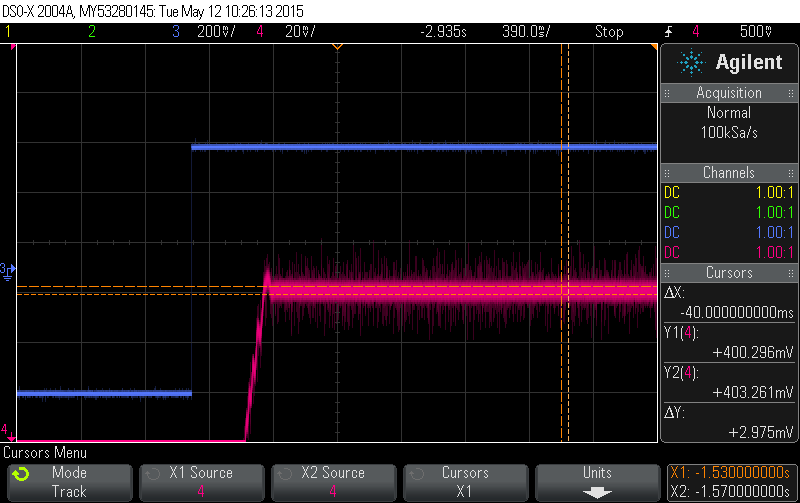
\includegraphics[width=0.5\linewidth]{Oscilloscope/PartC_Theoretical_Overshoot.png} 
			\caption{Theoretical Closed Loop Response}
			\label{fig:subim1}
	\end{figure}


WHAT WE CAN SEE FROM THIS (AS VOLTAGE GOES UP, THIS GOES UP) \\
Moreover, below is the recorded systems response after experimentally changing the resistor values, and hence the gain, to produce a 5\% overshoot. The experimental resistor values used to produce this overshoot were as follows; $R_1 = 10k$, $R_f = 62.8k \approx 56k + 6.8k$, resulting in a gain of $K = 6.28$. 

	\begin{figure}[H]
		\centering
		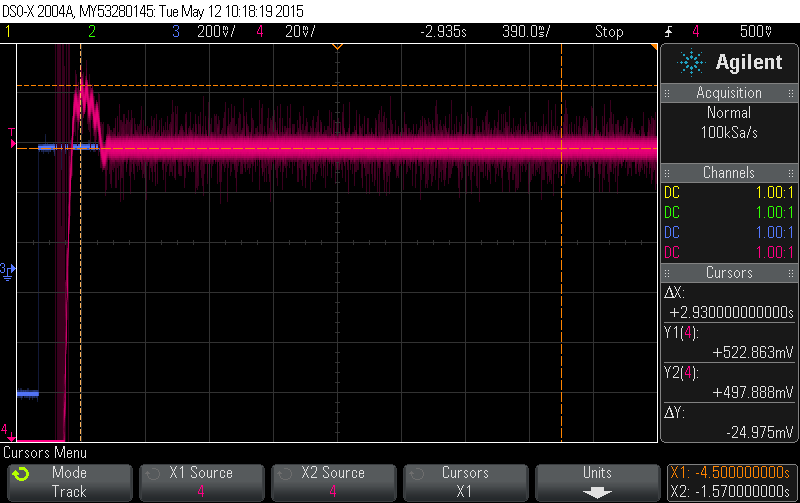
\includegraphics[width=0.5\linewidth]{Oscilloscope/PartC_Experimental_Overshoot.png}
		\caption{Experimental Closed Loop Response}
		\label{fig:subim2}
	\end{figure}

WHAT WE CAN SEE FROM THIS\\

compare models\\
compare gains\\
new method\\



closed loop control system for the position of the motor\\
overall TF\\
estimated gain for 5\% OS\\
practical gain for 5\% OS\\
comparisons\\
C8\\








\pagebreak
\subsection{Part D}
Experiment D explored the effect of input frequency on the closed loop system response, as well as examining the effect of increasing or decreasing the systems gain. \textcolor{red}{and bode}\\
  
\textcolor{red}{D1/C8} \\

After measuring and recording the systems response and percentage overshoot for five different input frequencies; the following table was constructed (refer to section~\ref{sec:d} for calculations responsible for the construction of this table). 

\begin{center}
    \begin{tabular}{| c | c |}
    \hline
    Input Frequency (Hz)  & Overshoot (\%)  \\ \hline
    0.5  	                  & 6.1  		\\ \hline
	0.75  	                  & 5.7  		\\ \hline
	1		                  & 6.1 		\\ \hline
	1.25	                  & 6.5 		\\ \hline
	1.5		                  & 5.8 		\\
    \hline
    \end{tabular}
\end{center}
 
Both the above table, and the systems response (figure~\ref{fig:freqimpact}) show clearly that increasing the frequency has no effect on overshoot, settling time, or steady state error. However, after the frequency exceeds a certain limit (\textbf{$1/f < Ts$}) the system does not have enough time to reach a steady state value. Moreover, if the frequency of the input where to continue increasing, eventually the operation amplifier will begin attenuating the output voltage. 

The reason the frequency has no effect on these values, as explained in section~\ref{sec:d}, is that the circuit contains no energy storing devices (such as capacitors or inductors), and as such- \textbf{frequency should not affect any circuit properties.} \textcolor{red}{Additionally, the approximated transfer function of this system is independent of the input frequency, or more simply;}
\begin{align*}
G_c(s) &= \frac{\frac{R_f}{R_1}K_m} {s^2 + s\alpha + \frac{R_f}{R_1}K_m}
\end{align*}
and recall, 
\begin{align*}
W_n &= \sqrt{b} = \sqrt{K_m * \frac{R_f}{R_1}} \\
\zeta &= \frac{a}{2b} = \frac{a}{2*W_n} = \frac{\alpha}{2*\sqrt{K_m * \frac{R_f}{R_1}}}
\end{align*}
and
\begin{align*}
\%OS &= e^{\frac{-\pi \zeta}{\sqrt{1-\zeta^2}}} * 100 \\
T_s &= \frac{4}{\zeta W_n}
\end{align*}

Thus, as neither $W_n$ or $\zeta$ are dependent on frequency, both overshoot and settling time are also independent of frequency. 
This explains why besides the reduced time available for the signal to settle, no visible changes to these properties were observed as the frequency was increased. 

The impact of the systems gain however, was much more noticeable. From figure~\ref{fig:gainimpact}, it can be seen that increasing the gain resulted in an increased overshoot and a decreased settling time. This has been proven more in depth in the associated answers section, but a summary of the findings can be found below.  \\
From the previous equations, it can be seen that both $\zeta$ and $W_n$ rely on the gain ($K = R_f/R_1$). Furthermore, this means both the overshoot and settling time rely on the gain factor.
\textbf{SUB IN TO FIND OS and Ts AND SHOW THEY RELY ON GAIN, PROP/invPROP}\\
\textbf{WHY IS THIS USEFUL - prop controller?}\\
\textcolor{red}{D4/D5}



\pagebreak
\section{Discussion/Recommendations:}
\textbf{0.5-1page}\\








\pagebreak
\section{Appendices}
\subsection{Pre-lab:}
\subsubsection{Lachlan Nicholson}
\textbf{PART A ANSWERS:}
\begin{enumerate}
	\item Below is the requested functional diagram for the complete servo motor control system.    
    \begin{figure}[H]
	\centering
	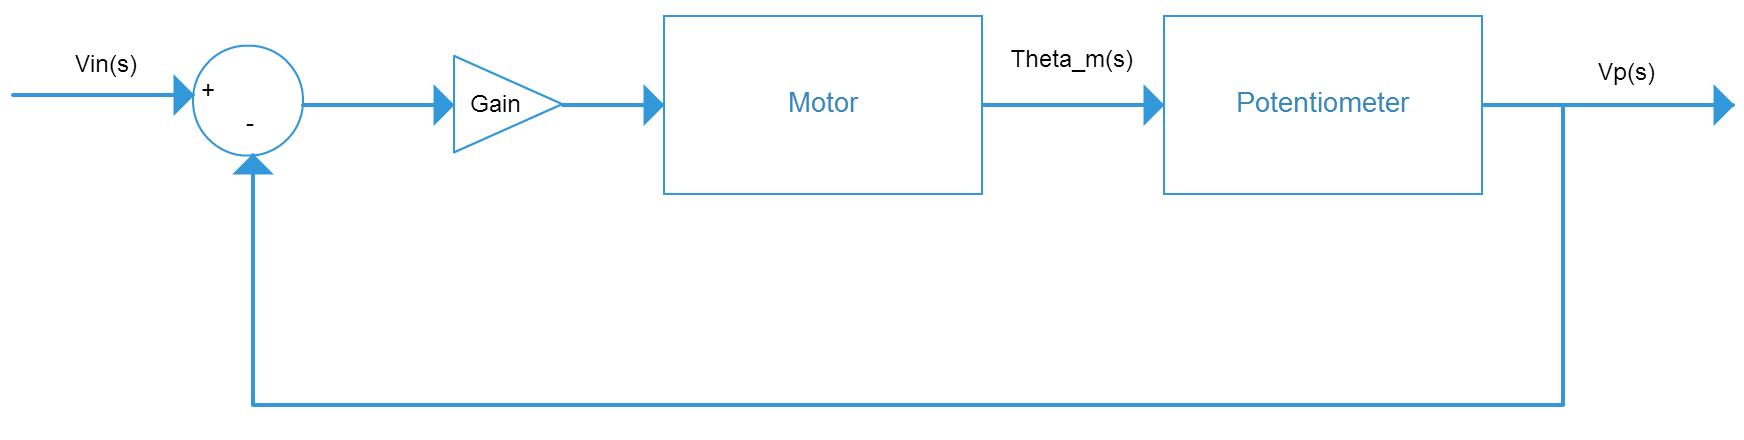
\includegraphics[width=.8\textwidth]{PreLach/A2a.png}
	\caption{\label{fig:funcagram}Functional Diagram of the control system}
	\end{figure}
    
    
	\item The updated functional diagram has been included below.
    \begin{figure}[H]
	\centering
	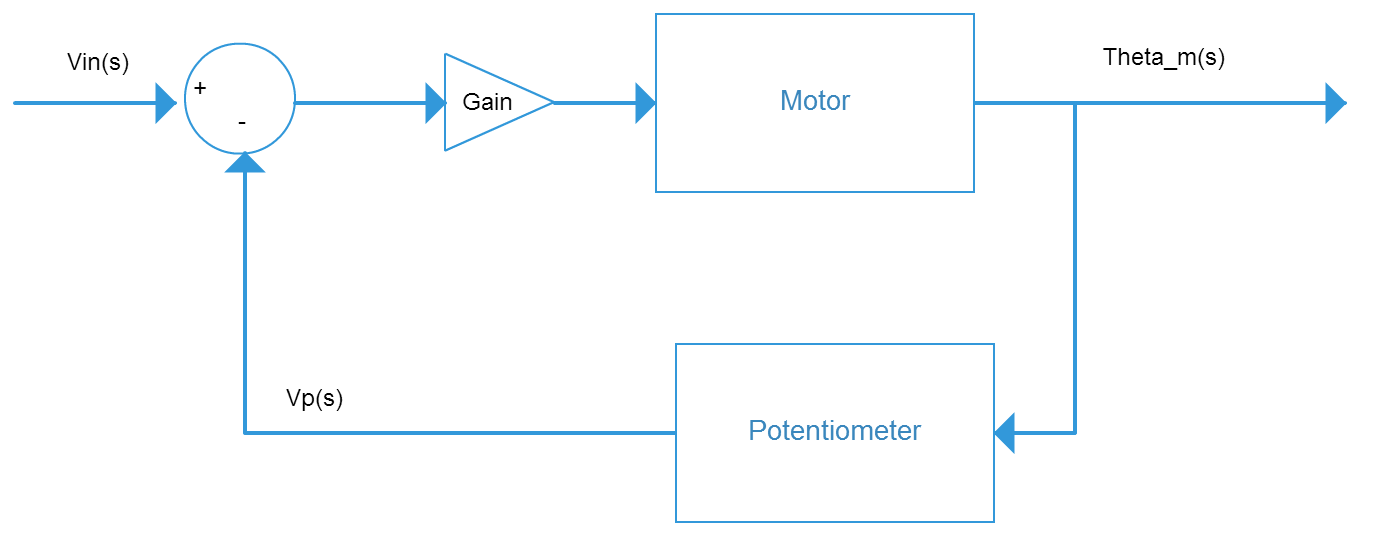
\includegraphics[width=.8\textwidth]{PreLach/A2b.png}
	\caption{\label{fig:updatedfuncagram}Updated Functional Diagram}
	\end{figure}
    
    
    
    
    \pagebreak
	\item The output of the requested matlab script has been included below, after which, the code itself has been provided. 
    \begin{figure}[H]
	\centering
	\includegraphics[width=.8\textwidth]{PreLach/a3.eps}
	\caption{\label{fig:simrep} Simulated Response}
	\end{figure}
    \begin{lstlisting}
%% A3
Alpha = 1;
K_m = 1;

t = linspace(0,10,100);
G_0 = tf([K_m],[1 Alpha 0]);
figure();
step(G_0, t, 'r')
print('-depsc','a3')
	\end{lstlisting}
    
    
    
    
    \pagebreak
	\item The given data describing the step response of an ideal servo model has been compared to the previously estimated system response. 
    \begin{figure}[H]
	\centering
	\includegraphics[width=.8\textwidth]{PreLach/a4.eps}
	\caption{\label{fig:datacomp}Given Data and Estimated Response}
	\end{figure}
    \begin{lstlisting}
%% A4    
Alpha = 1;
K_m = 1;
t = linspace(0,10,100);
G_0 = tf([K_m],[1 Alpha 0]);
    
load ENB301TestData_2015.mat
figure();
plot(t,y1);
hold;
step(G_0, t, 'r')
print('-depsc','a4')
	\end{lstlisting}
  
  
  
  
  
    \item \textbf{steady/transient Q}
    
    
    
    
    \pagebreak
    \item After changing the values of $K_m$ and $\alpha$ in the previous matlab script, it was found that values of $K_m = 1.3$ and $\alpha = 1$ resulted in an output that matched the test data. Furthermore, a script was created specifically to automatically find the best estimates for values of $K_m$ and $\alpha$ within a given range. The results of both the manual and automatic estimations have been included below. 
    \begin{figure}[H]
	\centering
	\includegraphics[width=.8\textwidth]{PreLach/a6a.eps}
	\caption{\label{fig:manest}Manually Estimated System Values}
	\end{figure}
    \begin{lstlisting}
%% A6
Alpha = 1; %0.5-1.5
K_m = 1.3; %1-2
G_0 = tf([K_m],[1 Alpha 0]);
figure();
plot(t,y1);
hold;
step(G_0, t, 'r');
print('-depsc','a6a')
	\end{lstlisting}
    
    \begin{figure}[H]
	\centering
	\includegraphics[width=.8\textwidth]{PreLach/a6b.eps}
	\caption{\label{fig:autoest}Inverting Amplifier System}
	\end{figure}
    \begin{lstlisting}
%% Automated:
% loop values of alpha and k_m
% calculate RMS error each time
% pick values with the least error

y1_rms = rms(y1);
prevdiff = 10000;

for Alpha = 0.1:0.1:3
    for K_m = 0.1:0.1:3
        G_0 = tf([K_m],[1 Alpha 0]);
        G_t = step(G_0, t, 'r');
        Gt_rms = rms(G_t);
        diff = y1_rms - Gt_rms;
        if (abs(diff) < abs(prevdiff))
            prevdiff = diff;
            K_m_f = K_m;
            Alpha_f = Alpha;
        end
    end
end

G_0 = tf([K_m_f],[1 Alpha_f 0]);
figure();
plot(t,y1);
hold;
step(G_0, t, 'r');
print('-depsc','a6b')

% Final values:
% Alpha_f = 1.3
% K_m_f = 1.7
    \end{lstlisting}
    
    
    
    
    
    
    \pagebreak
    \item Using matlabs random number generator, uncertainty was added to the output $y_1(t)$, and both the ideal and noisy response were plotted. \textbf{QUESTIONS}
    \begin{figure}[H]
	\centering
	\includegraphics[width=.8\textwidth]{PreLach/a7.eps}
	\caption{\label{fig:rand}Estimated System Response + Uncertainty}
	\end{figure}
    \begin{lstlisting}
%% A7
rand_power = 2;

y_1 = step(G_0, t, 'r');
y_n = y_1 + (rand_power/2)*rand(size(y_1,1),1) - (rand_power/2)*rand(size(y_1,1),1);

figure();
step(G_0, t, 'b');
hold;
plot(t,y_n,'r');
print('-depsc','a7')

	\end{lstlisting}
    
\end{enumerate}

\pagebreak
\textbf{PRELAB QUESTIONS:}
%% QUESTIONS:
% 1. 2
% 2. True
% 3. False, True, Increase Constantly, G_0(s)
% 4. data = data(527:end), calc = calc(100:end)
% 5. Divide 1st responce by gain of 1.38, or multiply with 2nd responce. 
\begin{enumerate}
	\item 2
	\item True
	\item False, True, Increase Constantly, $G_0(s)$
	\item data = data(527:end), calc = calc(100:end)
	\item Divide 1st response by gain of 1.38, or multiply with 2nd response. 
\end{enumerate}





\pagebreak
\subsubsection{Declan Gilmour}
\textbf{PART A ANSWERS:}
\begin{enumerate}
	\item \textbf{Model the complete servo motor control system using a functional diagram. Label all signals and assumptions made including measurement units.}
	\begin{figure}[H]
	\centering
	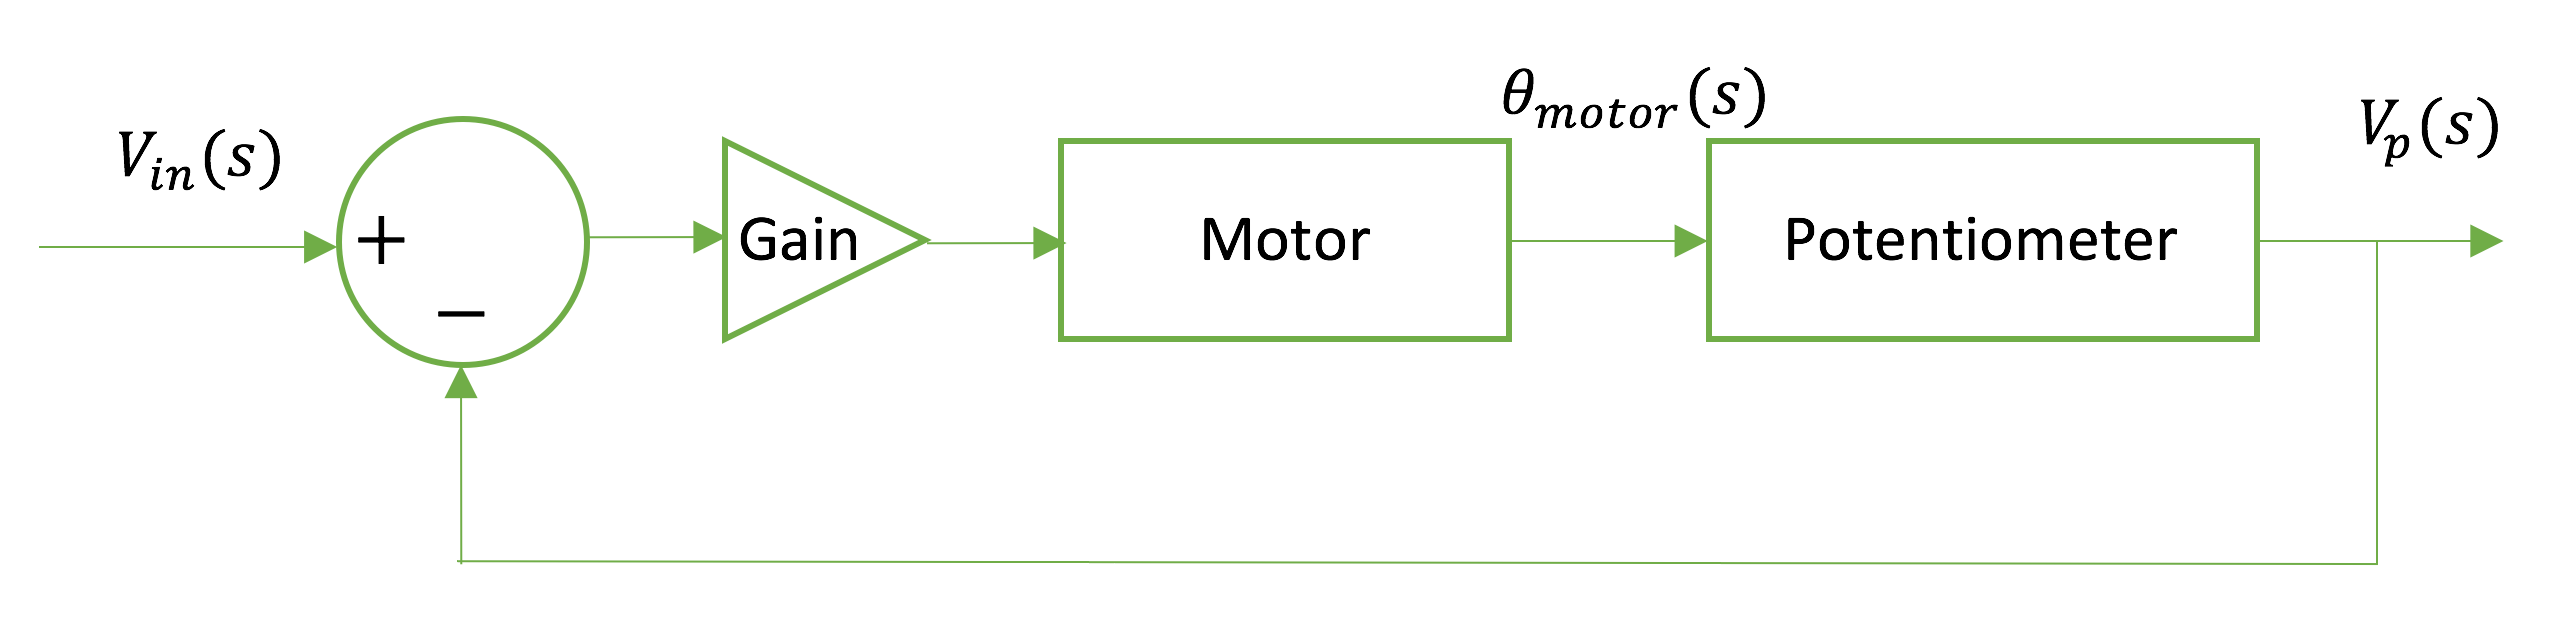
\includegraphics[width=.8\textwidth]{PreDec/A1.png}
	\caption{\label{fig:rand}Servo Motor Functional Diagram}
	\end{figure} 
	A voltage is fed into the motor with a magnitude gain. From here the voltage is converted into rotational movement $\theta_{motor}(s)$ by the motor.
	This rotational movement alters the displacement of the potentiometer wiper. The potentiometer acts as a sensor to indicate arm displacement in the form of output voltage $V_p(t)$.
	\item\textbf{Update the servo motor functional diagram and make any necessary changes.}
	\begin{figure}[H]
	\centering
	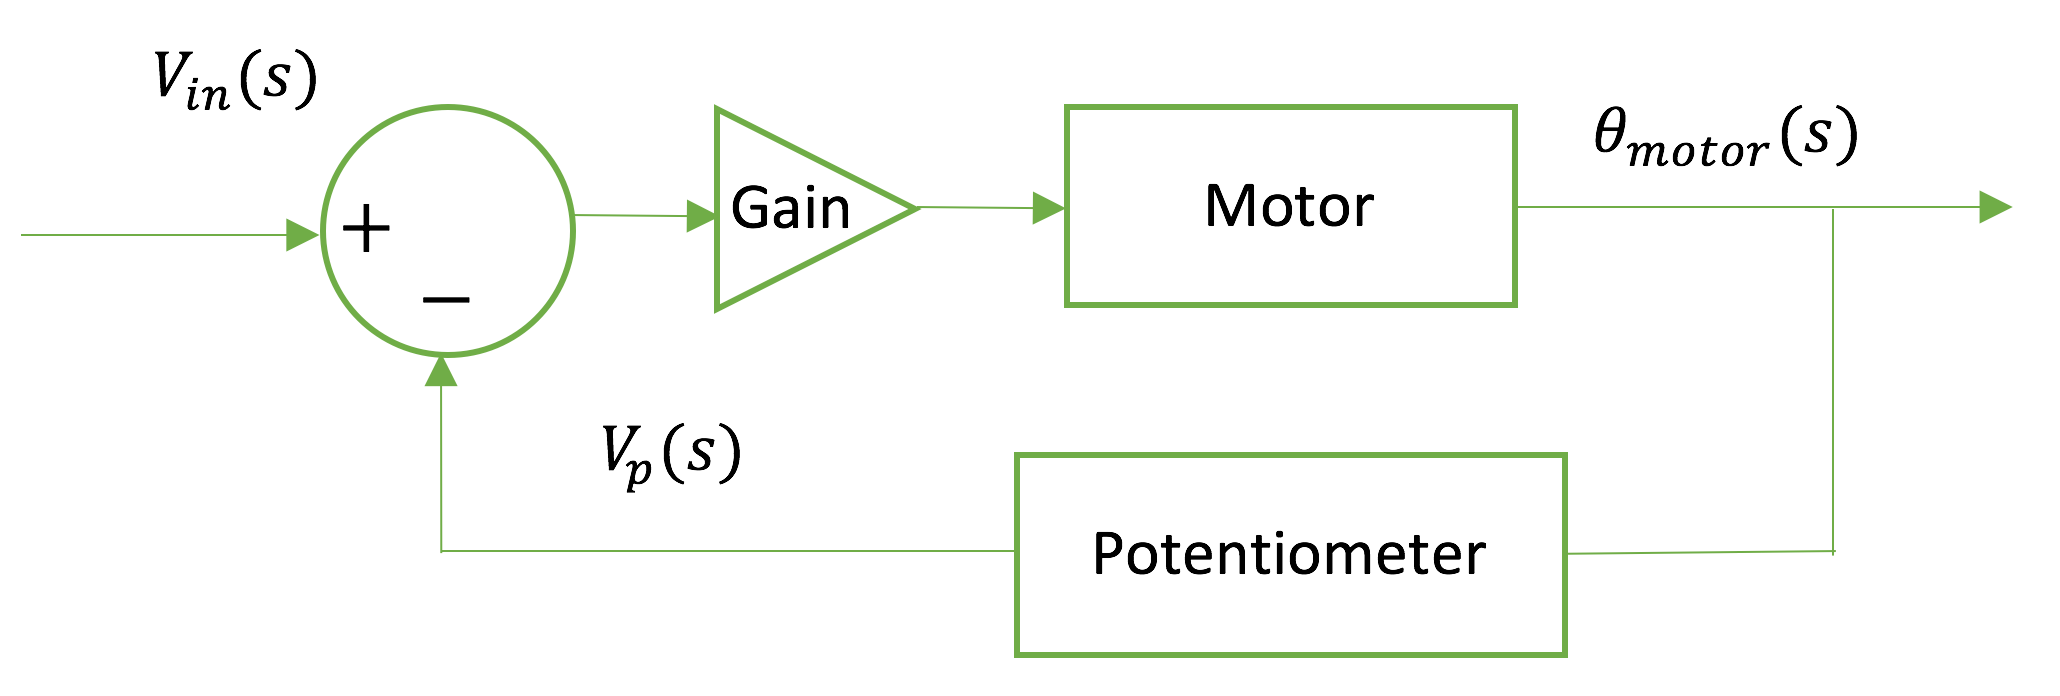
\includegraphics[width=.8\textwidth]{PreDec/A2.png}
	\caption{\label{fig:rand}Updated Servo Motor Functional Diagram}
	\end{figure}
	To calculate the two servo motor system characteristics, $\alpha$ and $K_m$ the system response would need to be recorded to a step input. This open loop time response is measured in terms of how the voltage applied to the motor affects the voltage seen at the potentiometer.\\
	The selection of optimum values of $\alpha$ and $K_m$, wold require the potentiometer voltage to be measured with respect of the input voltage. The modification of the Servo Motor Functional Diagram is needed, incorperating a feedback loop as shown.  
\pagebreak
	\item\textbf{Create code to simulate motor shaft angle for various values of $K_m$ and $\alpha$}\\
	Bellow is the Matlab code used to simulate the motor shaft angle.
	\begin{lstlisting}
%% A3 - Simulate motor shaft angle for values of km and alpha
alpha = 1;
km = 1;
t = linspace(0,10,100);

% Build transfer function
G = tf(km, [1 alpha 0]);    % Set G(s) = km / (s + a)  
G_0 = step(G,t);    % Set G_0(s) = km / (s * (s + a))

% Plot motor set response
figure
plot(t,G_0,'r')
title('Simulated Step Response')
xlabel('t (sec)')
ylabel('Amplitude')
print('-depsc','A3')
close
	\end{lstlisting}
	\begin{figure}[H]
	\centering
	\includegraphics[width=.8\textwidth]{PreDec/A3.eps}
	\caption{\label{fig:rand}Updated Servo Motor Functional Diagram}
	\end{figure}
\pagebreak
	\item\textbf{Plot $y_1(t)$ against the servo motor response in ENB301\_TestData and compare.} \\
	Bellow is the Matlab code used to generate the simulated step response against imported test data.
	\begin{lstlisting}
%% A4 - Plot motor unit step response data against simulated response
load ENB301TestData_2015.mat
alpha = 1;
km=1;
G = tf(km,[1 alpha 0]); 
G_0 = step(G,t);

figure
hold on
plot(t,y1,'b')
plot(t,G_0,'r')
title('Simulated Step Response and Test Data')
xlabel('t (sec)')
ylabel('Amplitude')
legend('y1(t): Simulated Step Response','Test Data')
hold off
print('-depsc','A4')
close
	\end{lstlisting}
	\begin{figure}[H]
	\centering
	\includegraphics[width=.8\textwidth]{PreDec/A4.eps}
	\caption{\label{fig:rand}Updated Servo Motor Functional Diagram}
	\end{figure}
\pagebreak
	\item\textbf{What is the steady state response and transient response predominantly determined by?}
\pagebreak
	\item\textbf{Change the values of $K_m$ and $\alpha$ for to match the simulated response with the test data.}\\
	The estimated $K_m$ value is 2.3838 and $\alpha$ 1.8990. Bellow is the Matlab Code to estimate km and alpha variables.
	\begin{lstlisting}
%% A6 - Estimate km and alpha variables
load ENB301TestData_2015
output = zeros(3,100*100);
error = 0;
ii = 1;
for km = linspace(0,4,100)
   for alpha = linspace(0,4,100)
       G = tf(km, [1 alpha 0]);
       G_0 = step(G,t);
       
       % Calculate mean square error
       for jj = 1 : length(t)
          error = error + (G_0(jj) - y1(jj))^2;
       end
       
       output(:,ii) = [km;alpha;error];
       ii = ii + 1;
       error = 0;
   end
end

[~,index] = min(output(3,:));
km = output(1,index); % Output variable
alpha = output(2,index);  % Output variable

% Build transfer function
G = tf(km, [1 alpha 0]);    % Set optimal G(s) = km / (s + a)   
G_0 = step(G,t);    % Set optimal G_0(s) = km / (s * (s + a))

% Plot step function G_0(s)
figure
hold on
plot(t,G_0,'-b');
plot(t,y1,'-r');
title('Estimated Step Response of Test Data')
xlabel('t (sec)')
ylabel('Amplitude')
legend('Estimated Step Response', 'Test Data');
hold off;
print('-depsc','A6')
close

% Output km and alpha
disp(km)    %2.3838
disp(alpha) %1.8990
	\end{lstlisting}
	\begin{figure}[H]
	\centering
	\includegraphics[width=.8\textwidth]{PreDec/A6.eps}
	\caption{\label{fig:rand}Estimated $K_m$ and $\alpha$ values}
	\end{figure}
\pagebreak
	\item\textbf{Plot the step response from original signal and a step response from a noisy signal.}\\
	Bellow is the Matlab Code to plot a step response from both original and noisy signals. $K_m = 2.4242$ and $\alpha = 1.9394$.

	\begin{lstlisting}
%load ENB301TestData_2015
% Generate noise
% Standard: sigma = 5, Decreased: signma = 0.2, Increased: sigma = 20
sigma = 5; %noise standard deviation
noise = sigma*randn(size(G_0)); %noise vector

% Create noisy signal
yn = y1 + noise;

output = zeros(3,100*100);
error = 0;
ii = 1;
for km = linspace(0,4,100)
   for alpha = linspace(0,4,100)
       G = tf(km, [1 alpha 0]);
       G_0 = step(G,t);
       
       % Calculate mean square error
       for jj = 1 : length(t)
          error = error + (G_0(jj) - yn(jj))^2;
       end
       
       output(:,ii) = [km;alpha;error];
       ii = ii + 1;
       error = 0;
   end
end

[~,index] = min(output(3,:));
km = output(1,index); % Output variable
alpha = output(2,index);  % Output variable

% Build transfer function
G_noisy = tf(km, [1 alpha 0]);    % Set optimal G(s) = km / (s + a)   
G_0_noisy = step(G_noisy,t);    % Set optimal G_0(s) = km / (s * (s + a))

% Output km and alpha
disp(km)    %2.4242
disp(alpha) %1.9394

% Plot noisy signal vs noisy test data
figure(2)
hold on
plot(t,G_0_noisy, '-r');
plot(t,G_0,'-b');
title('Estimated Step Response of Noisy Test Data')
xlabel('t (sec)')
ylabel('Amplitude')
legend('Noisy Step Response', 'Original Step Response');
hold off
print('-depsc','A7')
close
	\end{lstlisting}
	\begin{figure}[H]
	\centering
	\includegraphics[width=.8\textwidth]{PreDec/A7.eps}
	\caption{\label{fig:rand}Original Step Response and Noisy Step Response}
	\end{figure}
	For this noisy step response, $K_m = 1.4949$ and $\alpha = 1.1717$. When the noise noise decreases, $K_m$ and $\alpha$ decreases in magnitude. When the noise increases, $K_m$ and $\alpha$ increases in magnitude. The transient response of the system appears to increase as the noise of the system increases.\\\\
	\textbf{Is this Realistic?}\\\\
	\textbf{Whare are the source of uncertanty or noise in a real system?}\\
	Sources of uncertainty or noise in a system can include: control error, electrical noise, external factors such as weather and human error.
	\begin{figure}[H]	
		\begin{subfigure}{0.5\textwidth}
		\includegraphics[width=0.9\linewidth]{PreDec/A7_IncreasedNoise.eps} 
		\caption{Increased Noise: $K_m = 0.2828$ and $\alpha = 0.0808$}
		\label{fig:subim1}
		\end{subfigure}
		\begin{subfigure}{0.5\textwidth}
		\includegraphics[width=0.9\linewidth]{PreDec/A7_DecreasedNoise.eps}
		\caption{Decreased Noise: $K_m = 2.6263$ and $\alpha = 2.1010$}
		\label{fig:subim2}
		\end{subfigure}
  \caption{\label{fig:rand}Increased and Decreased noisey Step Response}
  \end{figure}

\end{enumerate}


\pagebreak
\textbf{PRELAB QUESTIONS:}










\pagebreak~\pagebreak
\subsection{Answers:}
\subsubsection{Part B}
\begin{enumerate}
	\item Read experimental data file(s) and store in vectors $y_e(t)$ and $t_e$. Plot the experimental results in black.
    
    \begin{lstlisting}
%% B1
% Load experimental data and plot in black
data = csvread('PartB_Test1.csv',2,0);  % Read in test 1
te_1 = data(1:end,1);   % Store te variable
te_1 = te_1 + abs(te_1(1)); % Move te variable to start at zero
ye_1 = data(1:end,2);   % Store ye variable
ye_1step = data(1:end,3);   % Store ye step input variable

figure
plot(te_1,ye_1,'k',te_1,ye_1step,'b')   % Plot ye in black and ye in blue
title('Experimental Data Plot [Set 1]')
xlabel('te (sec)')
ylabel('ye (voltage)')
print('-depsc',strcat('figures',filesep,'B1_dataset1'));    % Store figure
close
    \end{lstlisting}

	
    
  \begin{figure}[H]
	
  \begin{subfigure}{0.5\textwidth}
  \includegraphics[width=0.9\linewidth]{Matlab_Code/Figures/B1_dataset1.eps} 
  \caption{Data Set 1}
  \label{fig:subim1}
  \end{subfigure}
  \begin{subfigure}{0.5\textwidth}
  \includegraphics[width=0.9\linewidth]{Matlab_Code/Figures/B1_dataset2.eps}
  \caption{Data Set 2}
  \label{fig:subim2}
  \end{subfigure}
  
  \begin{subfigure}{0.5\textwidth}
  \includegraphics[width=0.9\linewidth]{Matlab_Code/Figures/B1_dataset3.eps}
  \caption{Data Set 3}
  \label{fig:subim3}
  \end{subfigure}

  \caption{\label{fig:rand}Open Loop response}
  \end{figure}

\pagebreak
	\item Modify the MATLAB script created in the pre-labs to simultaneously plot both the experimental data and $y_1(t)$.
    
    \begin{lstlisting}
%% B2
alpha = 1;
km=1;
G = tf(km,[1 alpha 0]);

G_0 = step(G,te_1);
figure
hold on
plot(te_1,G_0,'r')
plot(te_1,ye_1-ye_1(1),'b')
title('Simulated Step Response and Test Data')
xlabel('t (sec)')
ylabel('Amplitude')
legend('Simulated Step Response','Test Data')
hold off
print('-depsc',strcat('figures',filesep,'B2_dataset1'));
close
    \end{lstlisting}

   \begin{figure}[H]	
	  \begin{subfigure}{0.5\textwidth}
	  \includegraphics[width=0.9\linewidth]{Matlab_Code/Figures/B2_dataset1.eps} 
	  \caption{Data Set 1}
	  \label{fig:subim1}
	  \end{subfigure}
	  \begin{subfigure}{0.5\textwidth}
	  \includegraphics[width=0.9\linewidth]{Matlab_Code/Figures/B2_dataset2.eps}
	  \caption{Data Set 2}
	  \label{fig:subim2}
	  \end{subfigure}
	  
	  \begin{subfigure}{0.5\textwidth}
	  \includegraphics[width=0.9\linewidth]{Matlab_Code/Figures/B2_dataset3.eps}
	  \caption{Data Set 3}
	  \label{fig:subim3}
	  \end{subfigure}
  \caption{\label{fig:rand}Open Loop response}
  \end{figure}

	\item Derive a figure of merit for the estimation compared with experimental results.
    \\Mean Square error calculation: $error = (G_0 - y_e)^2$
    \\Root Mean Square error calculation: $error = \sqrt[2]{(G_0 - y_e))^2}$
	\item Improve estimates using the plots and figure of merit calculations. Derive the two parameters for the servo motor function $G(s) = \frac{K_m}{(S + \alpha)(S + \beta)}$.
  \begin{figure}[H]
	
  \begin{subfigure}{0.5\textwidth}
  \includegraphics[width=0.9\linewidth]{Matlab_Figures/B2_dataset1.eps} 
  \caption{Data Set 1}
  \label{fig:subim1}
  \end{subfigure}
  \begin{subfigure}{0.5\textwidth}
  \includegraphics[width=0.9\linewidth]{Matlab_Figures/B2_dataset2.eps}
  \caption{Data Set 2}
  \label{fig:subim2}
  \end{subfigure}
  
  \begin{subfigure}{0.5\textwidth}
  \includegraphics[width=0.9\linewidth]{Matlab_Figures/B2_dataset3.eps}
  \caption{Data Set 3}
  \label{fig:subim3}
  \end{subfigure}

  \caption{\label{fig:rand}Servo Motor Response Modified: $k_m$ and $\alpha$}
  \end{figure}
    

    \begin{lstlisting}
% Plot experimental data ye against systems estimated tf y1
[te_1new,ye_1new] = timing_fix(te_1,ye_1);
[te_2new,ye_2new] = timing_fix(te_2,ye_2);
[te_3new, ye_3new] = timing_fix(te_3,ye_3);

figure
plot(te_1new,ye_1new,'k')
title('Experimental Data Plot [Set 1 Adjusted]')
xlabel('te (sec)')
ylabel('ye (voltage)')
print('-depsc',strcat('figures',filesep,'B2_dataset1'));
close

figure
plot(te_1new,ye_1new,'k')
title('Experimental Data Plot [Set 1 Adjusted]')
xlabel('te (sec)')
ylabel('ye (voltage)')
print('-depsc',strcat('figures',filesep,'B2_dataset1'));
close
	\end{lstlisting}
	
    \begin{lstlisting}
% Pepare experimental data for alpha and km parameter calculations
[te_1trim, ye_1trim] = trimForCalculation(te_1new,ye_1new,mf1);
[te_2trim, ye_2trim] = trimForCalculation(te_2new,ye_2new,mf1);
[te_3trim, ye_3trim] = trimForCalculation(te_3new,ye_3new,mf1);

km_num = 500;    % number of km values used
km_max = 500;   % max km value used
alpha_num = 500;    % number of alpha values used
alpha_max = 500;    % max alpha value used
	\end{lstlisting}
   
    \begin{lstlisting}
% Preallocate size for speed
output_ms = zeros(3,km_num*alpha_num);
output_rms = zeros(3,km_num*alpha_num);
km_ms = zeros(1,3);
alpha_ms = zeros(1,3);
km_rms = zeros(1,3);
alpha_rms = zeros(1,3);
        
for iteration = 1 : 3
    
    % Set te and ye based on iteration
    if (iteration == 1)        
        te = te_1trim;
        ye = ye_1trim;
    elseif (iteration == 2)
        te = te_2trim;
        ye = ye_2trim;
    else
        te = te_3trim;
        ye = ye_3trim;
    end      
    
    % Set cycle variables
    error_ms = 0;
    error_rms = 0;
    ii = 1;
    count = 0;
    
    for km = linspace(0,km_max,km_num)   % Cycle km values
       for alpha = linspace(0,alpha_max,alpha_num)  % Cycle alpha values
           G = tf(km, [1 alpha 0]);
           G_0 = step(G,te);

           % Calculate error
           for jj = 1 : length(te)
              % Calculate mean square error
              error_ms = error_ms + (G_0(jj) - ye(jj))^2;
              
              % Calculate root mean square error
              error_rms = error_rms + rms(G_0(jj) - ye(jj));
           end
           
           % Store km, alpha and the error taken to calculate
           output_ms(:,ii) = [km;alpha;error_ms];
           output_rms(:,ii) = [km;alpha;error_rms];
           
           % Reset cycle variables
           ii = ii + 1;
           error_ms = 0;
           error_rms = 0;
       end
       
       % Output km iterations
       %count = count + 1;       
       %fprintf('%d %s %d\n',count,'/',km_num);
    end

    % Calculate km and alpha values for mean square error calculation
    [~,index] = min(output_ms(3,:));
    km_ms(iteration) = output_ms(1,index); % Output variable
    alpha_ms(iteration) = output_ms(2,index);  % Output variable

    % Calculate km and alpha values for root mean square error calculation
    [~,index] = min(output_rms(3,:));
    km_rms(iteration) = output_rms(1,index); % Output variable
    alpha_rms(iteration) = output_rms(2,index);  % Output variable    
end
km_mean = (mean(km_ms) + mean(km_rms)) / 2;
alpha_mean = (mean(alpha_ms) + mean(alpha_rms)) / 2;
    \end{lstlisting}
    
    \begin{lstlisting}
% Plot y1 against ye
% Data Set 1
G = tf(km_ms(1), [1 alpha_ms(1) 0]);
y1_ms = step(G,te_1new);
figure
plot(te_1new,medfilt1(ye_1new,1),'k',te_1new,medfilt1(y1_ms,1),'b')
title('Experimental vs estimated TF [Set 1 Adjusted, mean square error]')
xlabel('te (sec)')
ylabel('y (voltage)')
legend('ye','y1')
print('-depsc',strcat('figures',filesep,'y1_dataset1_ms'));
close
    \end{lstlisting}
    The average constants found are as follows:
    $\alpha = 170.3407$
    $k_m = 422.0107$
    
   \begin{figure}[H]
	
  \begin{subfigure}{0.5\textwidth}
  \includegraphics[width=0.9\linewidth]{Matlab_Figures/y1_dataset1_ms.eps} 
  \caption{Data Set 1 (ms)}
  \label{fig:subim1}
  \end{subfigure}
  \begin{subfigure}{0.5\textwidth}
  \includegraphics[width=0.9\linewidth]{Matlab_Figures/y1_dataset1_rms.eps}
  \caption{Data Set 1 (rms)}
  \label{fig:subim2}
  \end{subfigure}
  
  
  \begin{subfigure}{0.5\textwidth}
   \includegraphics[width=0.9\linewidth]{Matlab_Figures/y1_dataset2_ms.eps} 
   \caption{Data Set 2 (ms)}
   \label{fig:subim1}
   \end{subfigure}
   \begin{subfigure}{0.5\textwidth}
   \includegraphics[width=0.9\linewidth]{Matlab_Figures/y1_dataset2_rms.eps}
   \caption{Data Set 2 (rms)}
   \label{fig:subim2}
   \end{subfigure}
  
   \begin{subfigure}{0.5\textwidth}
   \includegraphics[width=0.9\linewidth]{Matlab_Figures/y1_dataset3_ms.eps} 
   \caption{Data Set 3 (ms)}
   \label{fig:subim1}
   \end{subfigure}
   \begin{subfigure}{0.5\textwidth}
   \includegraphics[width=0.9\linewidth]{Matlab_Figures/y1_dataset3_rms.eps}
   \caption{Data Set 3 (rms)}
   \label{fig:subim2}
   \end{subfigure}
   \caption{\label{fig:fig_18}Servo Motor Response Modeled}
   \end{figure}
	\item 
	$K_m = 426.6867$ and $\beta = 0.0646$. When considering the general transfer function of input voltage $G(s) = \frac{K_m}{(s+\alpha)(s+\beta)}$, a very small $\beta$ value would turn this into the simplified input voltage to motor shaft transfeer function $G_o(s) = \frac{V_p(s)}{V_m(s)} = \frac{K_m}{s(s + \alpha)}$.\\\\
	Therefore, the $\beta$ value of 0.0646 suggests the original assumption of the simplified input voltage to motor shaft transfer function was correct. The useful approximation if $|\beta| < 10|\alpha|$ the transient response will be dominated by $\alpha$ satisfies this system.\\
	Values were found for $y_1(t) \approx y_2(t)$ as shown in Fig~\ref{fig:fig_18} and Fig~\ref{fig:fig_19} respectively.\\
	From these observations, it is evident the electrical constant $\beta$ is negligable in this system. 


	The mechanical constant $\alpha$ was found to be $\alpha = alpha_{mean}$. Using the second order equation $G(s) = \frac{K_m}{(S + \alpha)}$ new values of gain constant $k_m$ and electrical constant $\beta$. Values were found for $y_1(t) \approx y_2(t)$.
    The average constants found are as follows:
    $\beta = 0.0646$
    $k_m = 426.6867$
    
   \begin{figure}[H]
	
  \begin{subfigure}{0.5\textwidth}
  \includegraphics[width=0.9\linewidth]{Matlab_Figures/y2_dataset1_ms.eps} 
  \caption{Data Set 1 (ms)}
  \label{fig:subim1}
  \end{subfigure}
  \begin{subfigure}{0.5\textwidth}
  \includegraphics[width=0.9\linewidth]{Matlab_Figures/y2_dataset1_rms.eps}
  \caption{Data Set 1 (rms)}
  \label{fig:subim2}
  \end{subfigure}
  
  \begin{subfigure}{0.5\textwidth}
  \includegraphics[width=0.9\linewidth]{Matlab_Figures/y2_dataset2_ms.eps} 
  \caption{Data Set 2 (ms)}
  \label{fig:subim1}
  \end{subfigure}
  \begin{subfigure}{0.5\textwidth}
  \includegraphics[width=0.9\linewidth]{Matlab_Figures/y2_dataset2_rms.eps}
  \caption{Data Set 2 (rms)}
  \label{fig:subim2}
  \end{subfigure}
  
  \begin{subfigure}{0.5\textwidth}
  \includegraphics[width=0.9\linewidth]{Matlab_Figures/y2_dataset3_ms.eps} 
  \caption{Data Set 3 (ms)}
  \label{fig:subim1}
  \end{subfigure}
  \begin{subfigure}{0.5\textwidth}
  \includegraphics[width=0.9\linewidth]{Matlab_Figures/y2_dataset3_rms.eps}
  \caption{Data Set 3 (rms)}
  \label{fig:subim2}
  \end{subfigure}
    \caption{\label{fig:fig_19}Servo Motor Response Modeled: $k_m$ and $\beta$}
    \end{figure}
    
    \pagebreak
 \begin{lstlisting}
km_num = 500;    % number of km values used
km_max = 500;   % max km value used
beta_num = 50;    % number of alpha values used
beta_max = 1;    % max alpha value used

% Preallocate size for speed
output_ms = zeros(3,km_num*beta_num);
output_rms = zeros(3,km_num*beta_num);
km2_ms = zeros(1,3);
beta_ms = zeros(1,3);
km2_rms = zeros(1,3);
beta_rms = zeros(1,3);
    
for iteration = 1:3
    if(iteration == 1)
        te = te_1trim;
        ye = ye_1trim;
    elseif(iteration==2)
        te = te_2trim;
        ye = ye_2trim;
    else
        te = te_3trim;
        ye = ye_3trim;
    end
    
    % Set cycle variables
    error_ms = 0;
    error_rms = 0;
    ii = 1;
    count = 0;
    
    for km = linspace(0,km_max,km_num)   % Cycle km values
       for beta = linspace(0,beta_max,beta_num)  % Cycle alpha values
           G = tf(km, [1 (alpha_mean+beta) (alpha_mean*beta)]);
           G_0 = step(G,te);

           % Calculate error
           for jj = 1 : length(te)
              % Calculate mean square error
              error_ms = error_ms + (G_0(jj) - ye(jj))^2;

              % Calculate root mean square error
              error_rms = error_rms + rms(G_0(jj) - ye(jj));
           end

           % Store km, alpha and the error taken to calculate
           output_ms(:,ii) = [km;beta;error_ms];
           output_rms(:,ii) = [km;beta;error_rms];

           % Reset cycle variables
           ii = ii + 1;
           error_ms = 0;
           error_rms = 0;
       end

        % Output km iterations
       %count = count + 1;       
       %fprintf('%d %s %d\n',count,'/',km_num);
    end

    % Calculate km and alpha values for mean square error calculation
    [~,index] = min(output_ms(3,:));
    km2_ms(iteration) = output_ms(1,index); % Output variable
    beta_ms(iteration) = output_ms(2,index);  % Output variable

    % Calculate km and alpha values for root mean square error calculation
    [~,index] = min(output_rms(3,:));
    km2_rms(iteration) = output_rms(1,index); % Output variable
    beta_rms(iteration) = output_rms(2,index);  % Output variable 
end

km_mean2 = (mean(km_ms) + mean(km2_rms)) / 2;
beta_mean = (mean(beta_ms) + mean(beta_rms)) / 2;
    \end{lstlisting}
    
    \begin{lstlisting}
% Plot y2 against ye
% Data Set 1
G = tf(km2_ms(1), [1 (alpha_mean+beta_ms(1)) (alpha_mean*beta_ms(1))]);
y2_ms = step(G,te_1new);
figure
plot(te_1new,medfilt1(ye_1new,1),'k',te_1new,medfilt1(y2_ms,1),'b')
title('Experimental vs estimated TF [Set 1 Adjusted, mean square error]')
xlabel('te (sec)')
ylabel('y (voltage)')
legend('ye','y1')
print('-depsc',strcat('figures',filesep,'y2_dataset1_ms'));
close
    \end{lstlisting}
    
\end{enumerate}













\pagebreak
\subsubsection{Part C}
\label{sec:c}
\begin{enumerate}
	\item \textbf{Re-draw figure~\ref{fig:c1_2_} and place boxes around the set of components that  correspond to each functional element of the control system.} \\
    
	\begin{figure}[H]
	\centering
	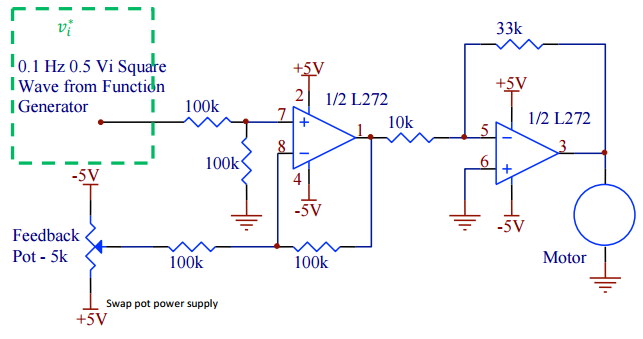
\includegraphics[width=.8\textwidth]{FigsC/c1_2_.png}
	\caption{\label{fig:c1_2_}Closed Loop Motor Control Schematic}
	\end{figure}
    
    \begin{figure}[H]
	\centering
	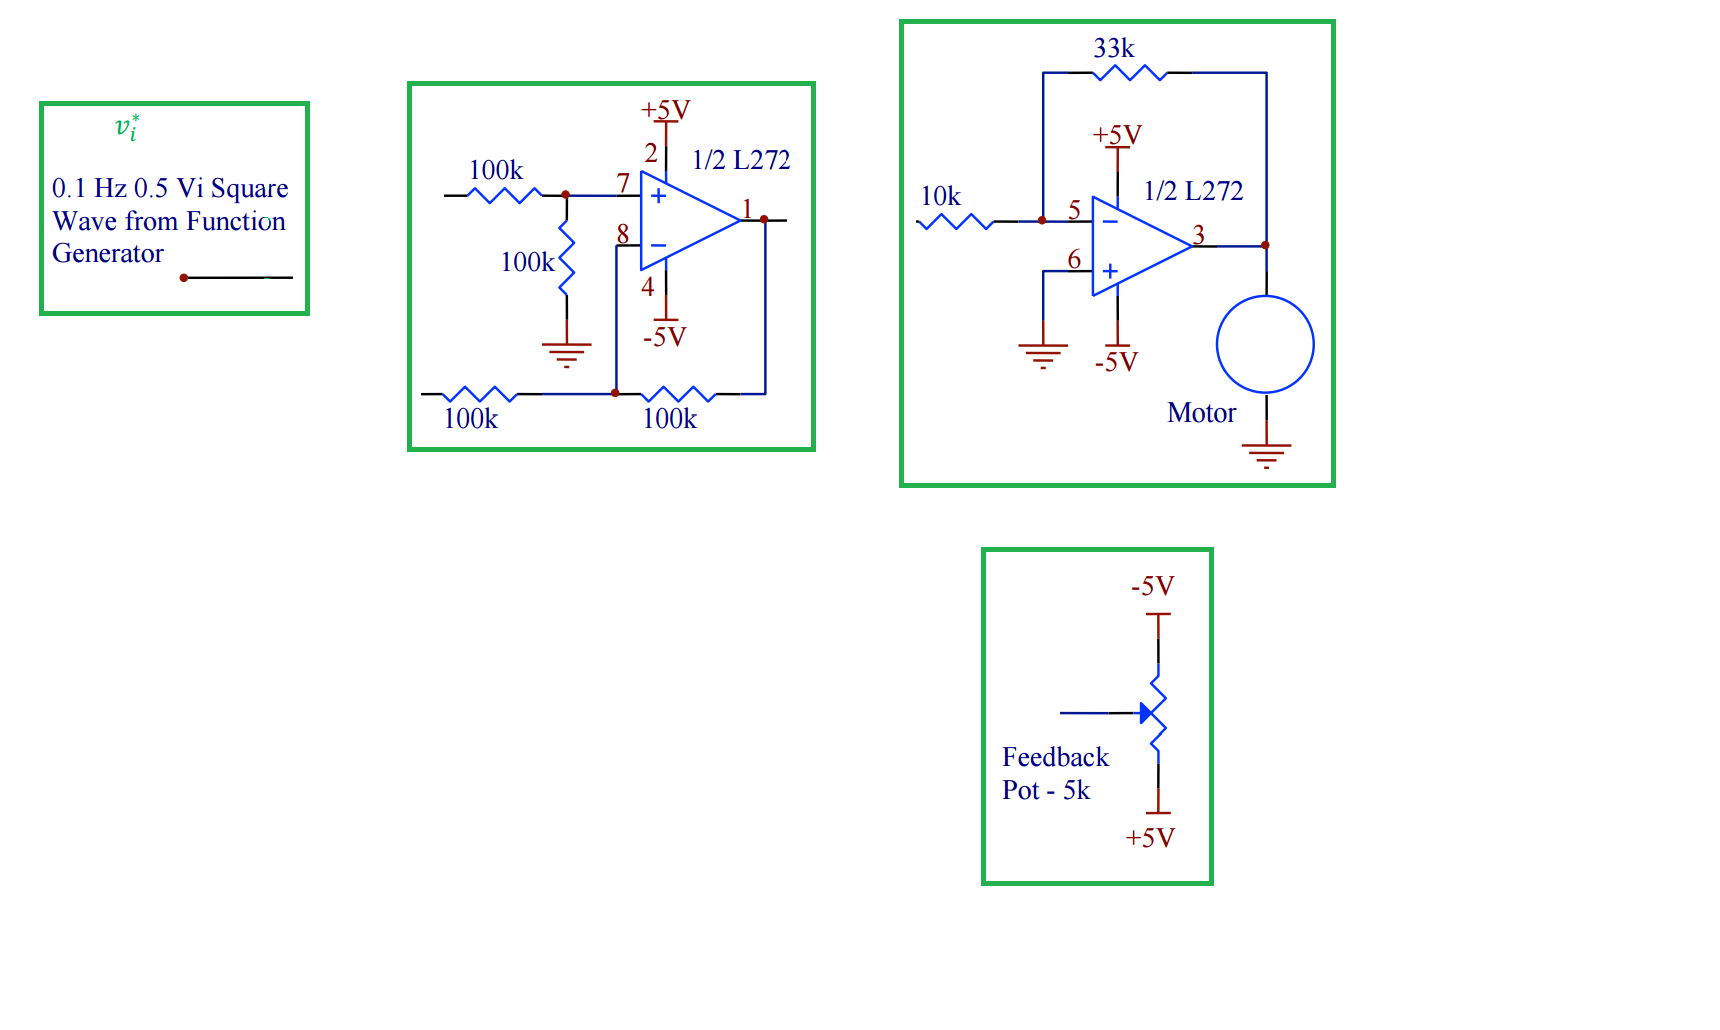
\includegraphics[width=.8\textwidth]{FigsC/c1.png}
	\caption{\label{fig:c1}Closed Loop Motor Control System}
	\end{figure}
    
    
    
    
    
    \pagebreak
	\item \textbf{Based on the results from Parts A and B, the component values given in figure~\ref{fig:c1_2_} and your research in parts C1, calculate all of the transfer functions in your functional diagram (figure~\ref{fig:c1}). Update the functional diagram, labeling all components and interfaces.}  \\
    
    \textbf{Difference Op-amp:}\\
    \begin{figure}[H]
    \centering
		\begin{subfigure}{0.4\textwidth}
		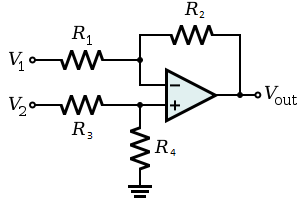
\includegraphics[width=1\textwidth]{FigsC/differenceOpAmp.png}
		\caption{Standard Difference Op Amp}
		\label{fig:subim1}
		\end{subfigure}
		\begin{subfigure}{0.5\textwidth}
		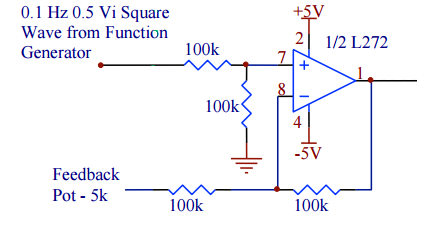
\includegraphics[width=1\textwidth]{FigsC/c2b.png}
		\caption{System Difference Op Amp}
		\label{fig:subim1}
		\end{subfigure}		
	\caption{\label{fig:diffamp}Difference Op-amp System}
	\end{figure}

    \begin{align*}
    \frac{V_{o}(s)}{V_{in}(s)} &= \frac{1+\frac{R_2}{R_1}}{1+\frac{R_3}{R_4}}V_2 - \frac{R_2}{R_1}V_1\\
	\frac{V_{o}(s)}{V_{in}(s)} &= V_{o}(s) - V_{p}(s)
	\end{align*}
    
    \textbf{Inverting Op-amp:}\\
    \begin{figure}[H]
    \centering
		\begin{subfigure}{0.4\textwidth}
		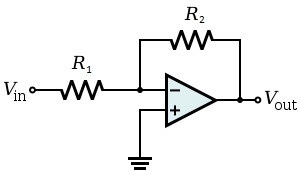
\includegraphics[width=1\textwidth]{FigsC/invertingOpAmp.png}
		\caption{Standard Difference Op Amp}
		\label{fig:subim1}
		\end{subfigure}
		\begin{subfigure}{0.4\textwidth}
		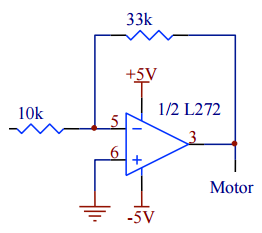
\includegraphics[width=1\textwidth]{FigsC/c2a.png}
		\caption{Inverting Op-amp System}
		\label{fig:subim1}
		\end{subfigure}		
	\caption{\label{fig:diffamp}Inverting Op-amp System}
	\end{figure}
    \begin{align*}
	\frac{V_{i}(s)}{V_{d}(s)} &= \frac{R_2}{R_1}
	\end{align*}\\
	Note: The polarity on the inverter transfer function has been flipped.
    
    \textbf{Motor:}\\
    \begin{align*}
	\frac{V_{p}(s)}{V_{i}(s)} &= \frac{K_m}{s(s+\alpha)}
	\end{align*}
	% \textbf{Motor and pot:}\\
	% \begin{align*}
	% \frac{V_{p}(s)}{V_{m}(s)} &= \frac{K_m}{s(s+\alpha)}
	% \end{align*}

    \begin{figure}[H]
	\centering
	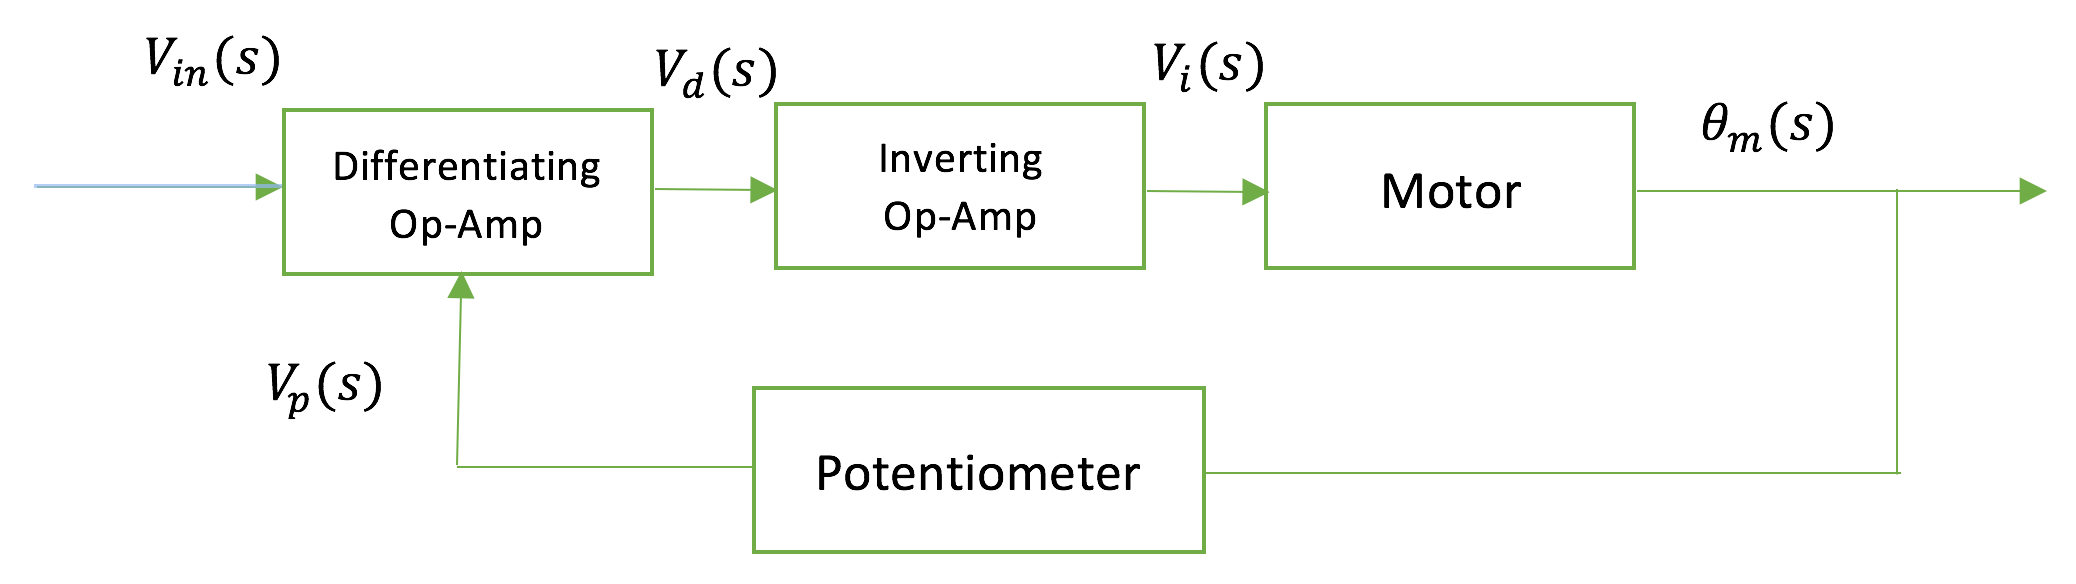
\includegraphics[width=.8\textwidth]{FigsC/c2c.png}
	\caption{\label{fig:c3}Updated Functional Diagram}
	\end{figure}

	
    

    
    
    
 %    \pagebreak
	% \item 
 %    \textbf{NONIDEAL:}\\
 %    \begin{align*}
	% V_{m}(s) &= \frac{R_2}{R_1} V_{1}(s) \\
 %    V_{m}(s) &= \frac{s(s+\alpha)}{K_m} V_{p}(s) \\
 %    \frac{R_2}{R_1} V_{1}(s) &= \frac{s(s+\alpha)}{K_m} V_{p}(s) \\
 %    V_{1}(s) &= \frac{R_1 s(s+\alpha)}{R_2 K_m} V_{p}(s) \\
 %    V_{1} &= 
	% \end{align*}
    
    
    
    
    
\pagebreak
\item Calculate the complete system transfer function $G_c(s)$. \\\\
\textbf{System Transfer Function:}\\
	\begin{align*}
	G_{c}(s) &= \frac{V_p(s)}{V_{in}(s)}\\ 
	&= \frac{V_p(s)}{V_i(s)}\times\frac{V_i(s)}{V_d(s)}\times\frac{V_d(s)}{V_{in}(s))}\\
	&= \frac{K_m}{s(s+\alpha)}\times\frac{R_2}{R_1}\times(V_i(s)-V_p(s))\\
	&=\frac{-K_m R_2}{R_1}\bigg(\frac{V_i(s)-V_p(s)}{s(s+\alpha)}\bigg)
	\end{align*}
From Inverting OP amp: $V_m(s) = \frac{R_2}{R_2}\times V_o(s)$\\\\
From Motor: $V_m(s) = \frac{s(s+\alpha)V_p(s)}{K_m}$
	\begin{align*}
	\therefore\frac{s(s+\alpha)V_p(s)}{K_m} &= \frac{R_2}{R_2}\times V_o(s)\\	
	V_o(s) &= \frac{R_1s(s+\alpha)}{K_mR_2}V_p(s)	\
	\end{align*}
From Difference Op Amp: $V_o(s) = V_i(s) - V_p(s)$
	\begin{align*}
	\therefore\frac{R_1s(s+\alpha)}{K_mR_2}V_p(s) &= V_i(s) - V_p(s)\\	
	V_p(s)\bigg[1-\frac{R_1s(s+\alpha)}{K_mR_2}\bigg] &= V_i(s)\\
	\frac{V_p(s)}{V_i(s)} &= \frac{1}{1+\frac{R_1s(s+\alpha)}{K_mR_2}}\\\\
	&= \frac{1}{1+\frac{R_1}{K_mR_2}(s^2+\alpha s)}\\\\
	&= \frac{1}{(\frac{R_1}{K_mR_2})s^2(\frac{\alpha R_1}{K_mR_2})s+1}\\\\
	&= \frac{\frac{K_m R_2}{R_1}}{s^2+(\frac{\alpha R_1 K_m R_2}{K_m R_2 R_1})s+\frac{K_m R_2}{R_1}}\\\\
	&= \frac{\frac{K_m R_2}{R_1}}{s^2+\alpha s+\frac{K_m R_2}{R_1}}
	\end{align*}	  

\pagebreak
    \textbf{Ideal System Transfer Function:}\\
    \begin{align*}
    G_c(s) &= \frac{K G(S)}{1 + K G(s) H(s)} \\\\
    G(s) &= \frac{K_m}{s(s+\alpha)} \\
    H(s) &= 1 \\
    K &= \frac{R_f}{R_1} \\\\
    G_c(s) &= \frac{\frac{R_f}{R_1} G(s)} {1 + \frac{R_f}{R_1} G(s)} \\
    G_c(s) &= \frac{\frac{R_f}{R_1} \frac{K_m}{s(s+\alpha)}} {1 + \frac{R_f}{R_1} \frac{K_m}{s(s+\alpha)}} \\
    G_c(s) &= \frac{\frac{\frac{R_f}{R_1}K_m}{s(s+\alpha)}} {1 + \frac{\frac{R_f}{R_1}K_m}{s(s+\alpha)}} \\
    G_c(s) &= \frac{\frac{R_f}{R_1}K_m} {s(s+\alpha) + \frac{R_f}{R_1}K_m} \\
    G_c(s) &= \frac{\frac{R_f}{R_1}K_m} {s^2 + s\alpha + \frac{R_f}{R_1}K_m}
	\end{align*}
    
    As can be seen, both the of the above methods produce the same result, the first requiring more complex algebra and all of the calculated transfer functions; the second method understands that the summing amplifier and inverting amplifier can be modeled as a summing node and gain block respectively (refer to figure~\ref{fig:updatedfuncagram}).
    
    From previously, $K_m = 326$, $\alpha = 38.61$, $R_f = 33k$ and $R_1 = 10k$.
    Thus,
    
    \begin{align*}
	G_c(s) &= \frac{\frac{33000}{10000}K_m} {s^2 + s\alpha + \frac{33000}{10000}K_m} \\
    G_c(s) &= \frac{3.3*K_m} {s^2 + s\alpha + 3.3*K_m} \\
    G_c(s) &= \frac{3.3*326} {s^2 + 38.61s + 3.3*326} \\
    G_c(s) &= \frac{1075.8} {s^2 + 38.61s + 1075.8} \\
	\end{align*}
    
    
    
    
    
    
    
    
    
    
	\item
	\textbf{$G_c(s) = \frac{1075.8} {s^2 + 38.61s + 1075.8}$ has been used to produce the expected time responce $y_c(t)$ of this system. The calculated characteristics are as follows:}\\
	Damping ratio (zeta): 0.690107\\
	Natural frequency (Wn): 27.973934\\
	Peak time (Tp): 0.155179\\
	\%OS (Mp): 0.050000\\
	Settling Time (Ts): 0.207200
    
    
    
    
    
    
    
    
    \pagebreak
	\item \textbf{Calculate the gain required in the final stage to produce a 5\% overshoot. Choose resistor values to match the required gain.} \\\\
    Recall, for 5\% overshoot, $\zeta = \frac{-\ln(5/100)}{\sqrt[]{\pi^2+\ln^2(5/100)}} = 0.69$\\
    And, the systems estimated overall transfer function; $\frac{k_m\frac{R_f}{R_1}}{s^2 + s\alpha + k_m\frac{R_f}{R_1}}$\\
    Whereas, the general second order transfer function; $\frac{W_n^2}{s^2 + 2\zeta W_n s + W_n^2}$\\
    Moreover, 
    \begin{align*}
	\alpha &= 2\zeta W_n\\
    W_n &= \frac{\alpha}{2\zeta}
	\end{align*}
    \begin{align*}
	W_n^2 &= k_m\frac{R_f}{R_1}\\
    \frac{R_f}{R_1} &= W_n^2/k_m\\
    K &= (\frac{\alpha}{2\zeta})^2/k_m
	\end{align*}
    
    From section B, we know $k_m = 326$ and $\alpha = 38.61$. We also calculated the required $\zeta$ previously, as 0.69. 
    \begin{align*}
    K &= (\frac{38.61}{2*0.69})^2/326\\
    K &= 2.4
	\end{align*}
    
    Therefore, the gain required to achieve a 5\% overshoot is as stated above; Moreover, to calculate the desired resistor values to achieve this game, we must make an initial assumption about either $R_f$ or $R_1$. \\
    Assuming $R_1 = 10k$ (as to avoid changing both resistors);
    \begin{align*}
    K &= 2.4 \\
    \frac{R_f}{R_1} &= 2.4 \\
    R_f &= 2.4*R_1 \\
    R_f &= 2.4*10 000 \\
    R_f &= 24 000 
	\end{align*}
    
    Thus, theoretically, to achieve 5\% overshoot a gain of $K = 2.4$ is required, to achieve this, $R_f = 24k \approx 22k + 1.8k + 220 = 24.2k$, and $R_1 = 10k$. 
    
%     Moreover, $W_n = \sqrt[]{b}$, $\zeta = \frac{a}{2b}$
%     \begin{align*}
% 	\zeta &= \frac{\alpha}{2*k_m\frac{R_f}{R_1}}\\
%     \zeta &= \frac{\alpha}{\frac{2*k_m*R_f}{R_1}}\\
%     \zeta &= \frac{\alpha*R_1}{2*k_m*R_f}\\
%     \zeta &= \frac{\alpha}{2*k_m} * \frac{R_1}{R_f}\\
%     \frac{R_f}{R_1} &= \frac{\alpha}{2*k_m*\zeta}\\
% 	\end{align*}
    
%     From section B, we know $k_m = 326$ and $\alpha = 38.61$. We also calculated the required $\zeta$ previously, as 0.69. 
    
%     \begin{align*}
%     \frac{R_f}{R_1} &= \frac{38.61}{2*326*0.69}\\
%     \frac{R_f}{R_1} = K &= \frac{38.61}{2*326*0.69}\\
% 	\end{align*}

	
    
    
    
    
\pagebreak    
	\item \textbf{Import experimental results into MATLAB. Compare your closed loop response data against your predicted model data $Y_c(t)$. Note any differences between the experimental result and the predicted result. What does this suggest about the model derived in part A and B?}
	\begin{figure}[H]
		\begin{subfigure}{0.5\textwidth}
		\includegraphics[width=0.9\linewidth]{Matlab_Code/Figures/C6_theoretical.eps} 
		\caption{Theoretical Closed Loop Response}
		\label{fig:subim1}
		\end{subfigure}
		\begin{subfigure}{0.5\textwidth}
		\includegraphics[width=0.9\linewidth]{Matlab_Code/Figures/C6_experimental.eps}
		\caption{Experimental Closed Loop Response}
		\label{fig:subim2}
		\end{subfigure} 
	\caption{\label{fig:rand}Servo Motor Closed Response}
	\end{figure}
	
	\begin{center}
		$\%OS = \frac{V_{max} - V_{avg}}{V_{avg}} \times 100$
	\end{center}
	\begin{align*}		
	    \%OS_{theoretical} &= \frac{403.261 - 400.296}{400.296} \times 100 \\
	    &= 0.7407\% \\\\
	    \%OS_{experimental} &= \frac{522.863 - 497.888}{497.888} \times 100 \\
	    &= 5.016\% 
	\end{align*}

	The motor response of the theoretical response was derived from $R_f = 25k$ ohms and $R_1 = 10k$ ohms with a calculated overshoot of 5\%. As shown in the calculations above, the theoretical percentage overshoot is much smaller. To obtain a 5\% overshoot, \\

    

    \pagebreak
	\item \textbf{Compare your experimentally derived 5\% overshot gain value against your predicted value. What is the percentage error? If your overshoot was too large for your derived gain value, could you use a controller other than the proportional controller to reduce overshoot? \\\\
If your steady state error was large, what other controller type could you use to minimize this error? What are  the drawbacks of  this  type of controller? What control applications can you think of that require very low steady state error?}\\

From the procedure outlined in \textbf{experiment C}, an experimental gain of $K = 6.28$ resulted in an overshoot of 5\%, and in \textbf{step 5} it was shown that the theoretical gain required to achieve this was $K = 2.4$.

The percentage error between the calculated and experimentally found gain values has been calculated below.
\begin{align*}
\%_{error} &= |\frac{K_{theoretical} - K_{experimental}}{K_{experimental}}| \times 100 \\
\%_{error} &= |\frac{6.28 - 2.4}{2.4}| \times 100 \\
\%_{error} &= 61.8\% 
\end{align*}
A large \% error value, as indicated above; provides strong evidence for model inaccuracies. The difference in gain between the theoretical and the practical values is likely caused losses that have been neglected from the simulation. \textbf{and we used the wrong values} 

The overshoot resulting from the derived gain value was under 5\%. 

Steady state error was noticeable in the system, likely caused by mechanical losses (gearbox, heat, etc). To alleviate this issue, a PI compensator (integrator) could be used; this is because the PI controller adds up error over time and would remove the steady state error. Moreover, a PI controller retains a maximum overshoot and settling time similar to that of the proportional controller (adjusting the gain alone). 

However, the drawbacks for a PI controller, depending on the application may include; the relatively faster settling time, or the possible overshoot, when compared to the effects of a PD controller.  

A good example of a control system that requires low steady state error is the cruise control on a car. This is largely to do with its specific application where the output were to be increased beyond the target output due to stead state error, the result could be decremental to safety, cause injury or even fatality. Moreover, any overshoot in the response would also have the ability to incur the previously mentioned effects. However, the systems response time is arguably less important, in fact it is dispersible to have a slower response time to avoid a large acceleration which would result in larger forces acting upon the driver, and could even reduce the vehicles stability or traction.

As mentioned previously, a PI compensator would remove the steady state error, but a PID controller would be the likely choice for a cruise control system, as elements from both a PI and a PD controller are wanted. The lack of steady state error, and a longer settling time and no peak overshoot are all possible when using a PID controller (with a focus on the derivative element).

\textbf{Add the actual OS from prac/theo} \\

    
    
    
    
    
    
    
	\item \textcolor{red}{Another method of calculating TF? (bode)}
\end{enumerate}










\pagebreak
\subsubsection{Part D}
\label{sec:d}
\begin{enumerate}
	\item \textcolor{red}{ANOTHER METHOD}
	
	
	
	
	
	\item The overshoot was measured over five different input frequencies in order to determine the effect over varying the input signals frequency. The systems response to these signals was also recorded, and can be found as a set of graphical time domain plots below.
	\begin{figure}[H]
	  \begin{subfigure}{0.5\textwidth}
	  \includegraphics[width=0.9\linewidth]{Matlab_Code/Figures/D2_0_5Hz.eps} 
	  \caption{Closed loop time domain response to 0.5Hz input.}
	  \label{fig:subim1}
	  \end{subfigure}
	  \begin{subfigure}{0.5\textwidth}
	  \includegraphics[width=0.9\linewidth]{Matlab_Code/Figures/D2_0_75Hz.eps}
	  \caption{Closed loop time domain response to 0.75Hz input.}
	  \label{fig:subim2}
	  \end{subfigure}
	  
	  \begin{subfigure}{0.5\textwidth}
	  \includegraphics[width=0.9\linewidth]{Matlab_Code/Figures/D2_1_0Hz.eps}
	  \caption{Closed loop time domain response to 1Hz input.}
	  \label{fig:subim2}
	  \end{subfigure}
	  \begin{subfigure}{0.5\textwidth}
	  \includegraphics[width=0.9\linewidth]{Matlab_Code/Figures/D2_1_25Hz.eps}
	  \caption{Closed loop time domain response to 1.25Hz input.}
	  \label{fig:subim2}
	  \end{subfigure}
	  
	  \begin{subfigure}{0.5\textwidth}
	  \includegraphics[width=0.9\linewidth]{Matlab_Code/Figures/D2_1_50Hz.eps}
	  \caption{Closed loop time domain response to 1.5Hz input.}
	  \label{fig:subim2}
	  \end{subfigure}
	\caption{\label{fig:freqimpact}Systems response to various input frequencies.}
	\end{figure}
	
	\pagebreak
	The percentage overshoot was calculated using the cursors on the digital CRO machine to measure the peak overshoot and the steady state voltage (average). 
	$$ \%OS = \frac{V_{peak}-V_{average}}{V_{average}} $$
	\begin{align*}
	OS(0.5Hz) 	&= \frac{525-495}{495} = 6.1 	\\
	OS(0.75Hz) 	&= \frac{523-495}{495} = 5.7 	\\
	OS(1Hz) 	&= \frac{525-495}{495} = 6.1 	\\
	OS(1.25Hz) 	&= \frac{525-495}{495} = 6.1 	\\
	OS(1.5Hz) 	&= \frac{524-495}{495} = 5.8 	
	\end{align*}
	
	The results of this analysis can be found in the following table.
	
\begin{center}
    \begin{tabular}{| c | c |}
    \hline
    Input Frequency (Hz)  & Overshoot (\%)  \\ \hline
    0.5  	                  & 6.1  		\\ \hline
	0.75  	                  & 5.7  		\\ \hline
	1		                  & 6.1 		\\ \hline
	1.25	                  & 6.5 		\\ \hline
	1.5		                  & 5.8 		\\
    \hline
    \end{tabular}
\end{center}


	
	As can be seen almost immediately in the previous plots, as the frequency of the input signal is increased, the output has less time to reach a steady state value. %Moreover, once the time elapsed per input cycle is reduced below the settling time, \textbf{the steady state response of the system is lost, and only the transient response has enough time to be viewable.} \\
	Eventually, the increasing frequency limits the systems ability to reach a steady state value.\\
	
	It is also evident from the previous figures and tables, that neither the overshoot, settling time or the steady state error are effected; until eventually the system does not have enough time to reach a steady state value. In addition to this, were the frequency to keep increasing, eventually the op-amps physical components would not be able to switch fast enough, and the output would be attenuated.\\
	
	The frequency does not effect any of the aforementioned properties, because quite simply; \textcolor{red}{the transfer function to which these properties can be derived, is independent of frequency. Which is to be expected, as there are no energy storing components in the system (capacitors, inductors).} 

\begin{figure}[H]
  \begin{subfigure}{0.5\textwidth}
  \includegraphics[width=0.95\linewidth]{Oscilloscope/PartD_0_5Hz_Overshoot.png} 
  \caption{Overshoot 0.5Hz}
  \label{fig:subim1}
  \end{subfigure}	  
  \begin{subfigure}{0.5\textwidth}
  \includegraphics[width=0.95\linewidth]{Oscilloscope/PartD_0_75Hz_Overshoot.png}
  \caption{Overshoot 0.75Hz}
  \label{fig:subim2}
  \end{subfigure}
  
  \begin{subfigure}{0.5\textwidth}
  \includegraphics[width=0.95\linewidth]{Oscilloscope/PartD_1_0Hz_Overshoot.png}
  \caption{Overshoot 1Hz}
  \label{fig:subim2}
  \end{subfigure}
  \begin{subfigure}{0.5\textwidth}
  \includegraphics[width=0.95\linewidth]{Oscilloscope/PartD_1_25Hz_Overshoot.png}
  \caption{Overshoot 1.25Hz}
  \label{fig:subim2}
  \end{subfigure}

  \begin{subfigure}{0.5\textwidth}
  \includegraphics[width=0.95\linewidth]{Oscilloscope/PartD_1_50Hz_Overshoot.png}
  \caption{Overshoot 1.5Hz}
  \label{fig:subim2}
  \end{subfigure}
\caption{\label{fig:freqimpact}Oscilloscope Overshoot Measurements}
\end{figure}

\begin{figure}[H]
  \begin{subfigure}{0.5\textwidth}
  \includegraphics[width=0.95\linewidth]{Oscilloscope/PartD_0_5Hz_SSE.png}
  \caption{SSE 0.5Hz}
  \label{fig:subim2}
  \end{subfigure}	  
  \begin{subfigure}{0.5\textwidth}
  \includegraphics[width=0.95\linewidth]{Oscilloscope/PartD_0_75Hz_SSE.png}
  \caption{SSE 0.75Hz}
  \label{fig:subim2}
  \end{subfigure}
 
  \begin{subfigure}{0.5\textwidth}
  \includegraphics[width=0.95\linewidth]{Oscilloscope/PartD_1_0Hz_SSE.png}
  \caption{SSE 1Hz}
  \label{fig:subim2}
  \end{subfigure}
  \begin{subfigure}{0.5\textwidth}
  \includegraphics[width=0.95\linewidth]{Oscilloscope/PartD_1_25Hz_SSE.png}
  \caption{SSE 1.25Hz}
  \label{fig:subim2}
  \end{subfigure}

  \begin{subfigure}{0.5\textwidth}
  \includegraphics[width=0.95\linewidth]{Oscilloscope/PartD_1_50Hz_SSE.png}
  \caption{SSE 1.5Hz}
  \label{fig:subim2}
  \end{subfigure}
\caption{\label{fig:freqimpact}Oscilloscope SSE Measurements}
\end{figure}

	
	
	
	
	
	
	
	
	\pagebreak
	\item To examine the impact of changing the gain value, the systems response data has been captured, recorded, and displayed below.
	\begin{figure}[H]
	  \begin{subfigure}{0.5\textwidth}
	  \includegraphics[width=0.95\linewidth]{Oscilloscope/PartD3_22k.png} 
	  \caption{Oscilloscope System Response to low gain ($R_f = 22k ohms$).}
	  \label{fig:subim1}
	  \end{subfigure}
	  \begin{subfigure}{0.5\textwidth}
	  \includegraphics[width=0.95\linewidth]{Oscilloscope/PartD3_100k.png}
	  \caption{Oscilloscope System Response to high gain ($R_f = 100k ohms$).}
	  \label{fig:subim2}
	  \end{subfigure}
	  \caption{\label{fig:gainimpact}Systems response to various gain values.}
	\end{figure}

	\begin{figure}[H]
	  \begin{subfigure}{0.5\textwidth}
	  \includegraphics[width=0.95\linewidth]{Matlab_Code/Figures/D3_22k.eps} 
	  \caption{Oscilloscope System Response to low gain.}
	  \label{fig:subim1}
	  \end{subfigure}
	  \begin{subfigure}{0.5\textwidth}
	  \includegraphics[width=0.95\linewidth]{Matlab_Code/Figures/D3_100k.eps}
	  \caption{Oscilloscope System Response to high gain.}
	  \label{fig:subim2}
	  \end{subfigure}
	  \caption{\label{fig:gainimpact}Systems response to various gain values.}
	\end{figure}
	
	As you would expect, changing the gain value \textbf{increases OS?} and \textbf{decreases Ts?}. The above images show large evidence to support this comment; as the correlation between these values can be seen clearly. \textbf{WHY}\\
	This is useful because \textbf{WHY}
\pagebreak
	\begin{lstlisting}
%% D3
data = csvread('PartD3_22k.csv',2,0);  % Read in 0.5Hz
td_22k = data(1:end,1);   % Store tc variable
%td_22k = td_22k + abs(td_22k(1));
yd_22k = data(1:end,3);   % Store yc variable
yd_22kStep = data(1:end,2);   % Store tc step input variable
[td_22k, yd_22k,yd_22kStep] = timing_fix_D3(td_22k,yd_22k,yd_22kStep);

figure
plot(td_22k,yd_22k,'k',td_22k,yd_22kStep,'b')
title('Time Response [Rf = 22k]')
xlabel('t (sec)')
ylabel('y (voltage)')
legend('Motor Response', 'Step input', 'Location','SouthEast')
print('-depsc',strcat('figures',filesep,'D3_22k'));
close

function [ te_new,ye_new, ye_stepNew ] = timing_fix_D3(te,ye,ye_step)
    te_new = te;
    ye_new = ye;
    ye_stepNew = ye_step;
    
    % Remove initial zero gradient before resonse
    f = ye_new > ye_new(1) * 1.05;
    indice = find(f,1,'first');
    ye_new = ye_new(indice-100:end);
    te_new = te_new(indice-100:end);
    ye_stepNew = ye_stepNew(indice-100:end);

    % Shift time to start at zero
    te_new = te_new + abs(te_new(1));

    % Shift amplitude to start at zero
    %ye_new = ye_new + ye_new(1);
end
	\end{lstlisting}
	
	
	
	
\pagebreak	
	\item 
	$G_c(s) = \frac{1075.8}{s^2 + 38.61s + 1075.8}$ has been used to produce the expected time response $y_c(t)$ of ths system.\\\\
	Damping ratio (zeta): 0.690107\\
	Natural frequency (Wn): 27.973934\\
	Peak time (Tp): 0.155179\\
	\%OS (Mp): 0.050000\\
	Settling Time (Ts): 0.207200
	\begin{lstlisting}
%% C4
%Calculate expected time response
Rf = 33 * 10^3;
R1 = 10 * 10^3;
alpha = 38.61;
Km = 326;
K = Rf / R1;

t = linspace(0,0.8,100);
G_c = tf(K * Km, [1 alpha K * Km]);
Y_c = 0.5 * step(G_c,t);

figure
plot(t,Y_c,'k')
title('Experimental vs estimated TF [Set 3 Adjusted, root mean square error]')
xlabel('te (sec)')
ylabel('Amplitude')
print('-depsc',strcat('figures',filesep,'C4'));
close

%Y_c = tf(K * Km, [1 alpha K * Km 0]);
num = 0.5 * K * Km;
den = [1 alpha K*Km 0];
% [num, den] = tfdata(Y_c,'v');
%r = gain, p = pole, k = direct term ie r / (s + p) + k
[r, p, k] = residue(num,den);
% 
syms s;
partialFrac = [r(1)/(s-p(1)) r(2)/(s-p(2)) r(3)/(s-p(3))];
time_response = ilaplace(partialFrac);  % Inverse laplace from s domain to t domain
time_response = vpa(time_response,5); % Round to 5 sig figs

zeta = -log(5/100) / sqrt(pi^2 +log(5/100)^2);  % Damping ratio
Wn = alpha / (2 * zeta);    % Natural frequency
Wd = Wn * sqrt(1 - zeta^2);
Tp = pi / Wd;   % Peak time
Mp = exp((-pi  * zeta) / sqrt(1 - zeta^2)); % Percentage overshoot
Ts =  4 / (zeta * Wn);   % Settling time
	\end{lstlisting}

	\begin{figure}[H]
	\centering
	\includegraphics[width=.8\textwidth]{Matlab_Code/Figures/C4.eps}

	\caption{\label{fig:funcagram}Time response of system.}
	\end{figure}

	\item \textbf{\textcolor{red}{C4 - Matlab - Declan?}} PD/PI/PID controller
\pagebreak 
\subsection{Prac Code}
This section contains all matlab code used during the practical lab. Lachlan Nicholson (n8866864) and Declan Gilmour (n8871566) worked in a prac group with Thomas Wagner (N8840121) and Antony Foster (N8647780).\\
\textbf{This code was produced by Thomas Wagner N8840121 and Antony Foster N8647780.}
\begin{lstlisting}
%------------B1. Loading data----------------------------%
[te,ye] = Data_cutting(closed,2,1);
[te,ye] = timing_fix(te,ye);
figure(i);i=i+1;
plot(te,ye,'k');
title('Test data plotted');
ylabel('Amplitude');
xlabel('Time_{sec}');

%------------B2 Plotting y2 and Experimental data---------%

Vm=1;
y3=step(G_1*Vm,te);
figure(i);i=i+1;
plot(te,y3,te,ye);
title('Test data Vs Calculated Km and Alpha ');
ylabel('Amplitude');
xlabel('Time_{sec}');

%-------------B3 Figure of merit-------------------------%
y_rms =@(x0)Variable_finder2(x0,'results.csv',te,ye);

%-------------B4 Recalculated values---------------------%

params = fminsearch(y_rms,[Km, a]);
y3_num =  [params(1)];
y3_den = [1 params(2) 0];
G_3 = tf(y3_num,y3_den)
y3= step(G_3*Vm,te);
 
figure(i);i=i+1;
plot(te,y3,te,ye);
title('Test data Vs ReCalculated Km and Alpha');
ylabel('Amplitude');
xlabel('Time_{sec}');
\end{lstlisting}
\end{enumerate}










\pagebreak
\section{CHECKLIST}
\begin{enumerate}
	\item Executive Summary
	\item Introduction
	\item Procedure Intro
	\item Procedure (D) - add new method
	\item \textcolor{green}{Results (B)}
	\item Results (C)
	\begin{enumerate}
		\item Is the transfer function as we'ed expect?
		\item \textcolor{green}{Closed loop response figures (theoretical gain or given gain?)}
		\item What can be seen from the figures
		\item \textcolor{green}{Experimental gain figures}
		\item What can be seen from this
		\item \textcolor{green}{Compare models}
		\item \textcolor{blue}{Compare gains}
		\item \textbf{NEW METHOD for finding TF}
	\end{enumerate}
	\item Results (D)
	\begin{enumerate}
		\item \textbf{DO NEW METHOD}
		\item \textcolor{blue}{Check tables peak overshoot}
		%\item \textcolor{blue}{Find word}
		%\item \textcolor{blue}{Check results are right (freq doesnt affect system)}
		\item \textcolor{blue}{Why is the effect of gain useful?}
		\item \textcolor{green}{SIMULINK MODEL}
		\item \textcolor{green}{PI/PD controller}
	\end{enumerate}
	\item \textbf{DISCUSSION and RECOMMENDATIONS}
	\item \textcolor{green}{Answers (B) - add more words?}
	\item Answers (C)
	\begin{enumerate}
		\item \textcolor{blue}{Fix figures}
		\item \textcolor{green}{Add non-ideal method}
		\item \textcolor{green}{C(4)}
		\item \textcolor{blue}{Finish C(7)}
		\item \textbf{NEW METHOD for finding TF}
	\end{enumerate}
	\item Answers (D) 
	\begin{enumerate}
		\item \textbf{DO NEW METHOD}
		\item \textcolor{blue}{Does frequency affect anything?}
		\item \textcolor{blue}{Prove how gain affects shit}
		\item \textcolor{green}{SIMULINK MODEL}
		\item \textcolor{green}{PI/PD controller}
	\end{enumerate}
\end{enumerate}






NOTES:
on first page, acknowledge assistance from students 
list group members / lab members


%\subsection{Exercise Alpha}




\end{document}